% version 1.2 dated 09 May 2011

% This file (c) 2009-2011 Elsevier Ltd.  Modifications may be freely made,
% provided the edited file is saved under a different name

% This file contains modifications for Procedia Computer Science

% Changes since version 1.1
% - added "procedia" option compliant with ecrc.sty version 1.2a
%   (makes the layout approximately the same as the Word CRC template)
% - added example for generating copyright line in abstract

%-----------------------------------------------------------------------------------

%% This template uses the elsarticle.cls document class and the extension package ecrc.sty
%% For full documentation on usage of elsarticle.cls, consult the documentation "elsdoc.pdf"
%% Further resources available at http://www.elsevier.com/latex

%-----------------------------------------------------------------------------------

%%%%%%%%%%%%%%%%%%%%%%%%%%%%%%%%%%%%%%%%%%%%%%%%%%%%%%%%%%%%%%
%%%%%%%%%%%%%%%%%%%%%%%%%%%%%%%%%%%%%%%%%%%%%%%%%%%%%%%%%%%%%%
%%                                                          %%
%% Important note on usage                                  %%
%% -----------------------                                  %%
%% This file should normally be compiled with PDFLaTeX      %%
%% Using standard LaTeX should work but may produce clashes %%
%%                                                          %%
%%%%%%%%%%%%%%%%%%%%%%%%%%%%%%%%%%%%%%%%%%%%%%%%%%%%%%%%%%%%%%
%%%%%%%%%%%%%%%%%%%%%%%%%%%%%%%%%%%%%%%%%%%%%%%%%%%%%%%%%%%%%%

%% The '3p' and 'times' class options of elsarticle are used for Elsevier CRC
%% The 'procedia' option causes ecrc to approximate to the Word template
\documentclass[3p,times,procedia]{elsarticle}
\flushbottom

%% The `ecrc' package must be called to make the CRC functionality available
\usepackage{ecrc}
%\usepackage{parskip}
\usepackage{amsmath}
\usepackage{ragged2e}
\usepackage{graphicx}
\usepackage{float}
\usepackage{listings}
\usepackage{color}
\usepackage{caption}
\usepackage{multicol}
\usepackage{titlesec}

\titleformat*{\section}{\Large\bfseries}
\titleformat*{\subsection}{\large\bfseries}
\titleformat*{\subsubsection}{\normalsize\bfseries}

\captionsetup[figure]{font=normalsize}

% \lstset{basicstyle=\ttfamily, keywordstyle=\bfseries}
\definecolor{mygreen}{rgb}{0,0.6,0}
\definecolor{mygray}{rgb}{0.5,0.5,0.5}
\definecolor{mymauve}{rgb}{0.58,0,0.82}

\lstset{ %
  backgroundcolor=\color{white},   % choose the background color
  basicstyle=\scriptsize,        % size of fonts used for the code
  breaklines=true,                 % automatic line breaking only at whitespace
  captionpos=b,                    % sets the caption-position to bottom
  commentstyle=\color{mygreen},    % comment style
  escapeinside={\%*}{*)},          % if you want to add LaTeX within your code
  keywordstyle=\color{blue},       % keyword style
  stringstyle=\color{mymauve},     % string literal style
}



\definecolor{darkred}{rgb}{0.6,0.0,0.0}
\definecolor{darkgreen}{rgb}{0,0.50,0}
\definecolor{lightblue}{rgb}{0.0,0.42,0.91}
\definecolor{orange}{rgb}{0.99,0.48,0.13}
\definecolor{grass}{rgb}{0.18,0.80,0.18}
\definecolor{pink}{rgb}{0.97,0.15,0.45}

% listings
\usepackage{listings}

% General Setting of listings
\lstset{
  aboveskip=1em,
  breaklines=true,
  abovecaptionskip=-6pt,
  captionpos=b,
  escapeinside={\%*}{*)},
  frame=single,
%   numbers=left,
  numbersep=15pt,
  numberstyle=\tiny,
}
% 0. Basic Color Theme
% \lstdefinestyle{colored}{ %
%   basicstyle=\ttfamily,
%   backgroundcolor=\color{white},
%   commentstyle=\color{green}\itshape,
%   keywordstyle=\color{blue}\bfseries\itshape,
%   stringstyle=\color{red},
% }
% 1. General Python Keywords List
\lstdefinelanguage{PythonPlus}[]{Python}{
  morekeywords=[1]{,as,assert,nonlocal,with,yield,self,True,False,None,} % Python builtin
  morekeywords=[2]{,__init__,__add__,__mul__,__div__,__sub__,__call__,__getitem__,__setitem__,__eq__,__ne__,__nonzero__,__rmul__,__radd__,__repr__,__str__,__get__,__truediv__,__pow__,__name__,__future__,__all__,}, % magic methods
  morekeywords=[3]{,object,type,isinstance,copy,deepcopy,zip,enumerate,reversed,list,set,len,dict,tuple,range,xrange,append,execfile,real,imag,reduce,str,repr,}, % common functions
  morekeywords=[4]{,Exception,NameError,IndexError,SyntaxError,TypeError,ValueError,OverflowError,ZeroDivisionError,}, % errors
  morekeywords=[5]{,ode,fsolve,sqrt,exp,sin,cos,arctan,arctan2,arccos,pi, array,norm,solve,dot,arange,isscalar,max,sum,flatten,shape,reshape,find,any,all,abs,plot,linspace,legend,quad,polyval,polyfit,hstack,concatenate,vstack,column_stack,empty,zeros,ones,rand,vander,grid,pcolor,eig,eigs,eigvals,svd,qr,tan,det,logspace,roll,min,mean,cumsum,cumprod,diff,vectorize,lstsq,cla,eye,xlabel,ylabel,squeeze,}, % numpy / math
}
% 2. New Language based on Python
\lstdefinelanguage{PyBrIM}[]{PythonPlus}{
  emph={d,E,a,Fc28,Fy,Fu,D,des,supplier,Material,Rectangle,PyElmt},
}
% 3. Extended theme
\lstdefinestyle{colorEX}{
  basicstyle=\ttfamily,
  backgroundcolor=\color{white},
  commentstyle=\color{darkgreen}\slshape,
  keywordstyle=\color{blue}\bfseries\itshape,
  keywordstyle=[2]\color{blue}\bfseries,
  keywordstyle=[3]\color{grass},
  keywordstyle=[4]\color{red},
  keywordstyle=[5]\color{orange},
  stringstyle=\color{darkred},
  emphstyle=\color{pink}\underbar,
}



\newcommand{\subf}[2]{%
  {\small\begin{tabular}[t]{@{}c@{}}
  #1\\#2
  \end{tabular}}%
}

%% The ecrc package defines commands needed for running heads and logos.
%% For running heads, you can set the journal name, the volume, the starting page and the authors

%% set the volume if you know. Otherwise `00'
%%\volume{}

%% set the starting page if not 1
\firstpage{1}

%% Give the name of the journal
\journalname{Computational Intelligence, Spring 2022}

%% Give the author list to appear in the running head
%% Example \runauth{C.V. Radhakrishnan et al.}
\runauth{}

%% The choice of journal logo is determined by the \jid and \jnltitlelogo commands.
%% A user-supplied logo with the name <\jid>logo.pdf will be inserted if present.
%% e.g. if \jid{yspmi} the system will look for a file yspmilogo.pdf
%% Otherwise the content of \jnltitlelogo will be set between horizontal lines as a default logo

%% Give the abbreviation of the Journal.
%% \jid{}

%% Give a short journal name for the dummy logo (if needed)
%\jnltitlelogo{Computer Science}

%% Hereafter the template follows `elsarticle'.
%% For more details see the existing template files elsarticle-template-harv.tex and elsarticle-template-num.tex.

%% Elsevier CRC generally uses a numbered reference style
%% For this, the conventions of elsarticle-template-num.tex should be followed (included below)
%% If using BibTeX, use the style file elsarticle-num.bst

%% End of ecrc-specific commands
%%%%%%%%%%%%%%%%%%%%%%%%%%%%%%%%%%%%%%%%%%%%%%%%%%%%%%%%%%%%%%%%%%%%%%%%%%

%% The amssymb package provides various useful mathematical symbols

\usepackage{amssymb}
%% The amsthm package provides extended theorem environments
%% \usepackage{amsthm}

%% The lineno packages adds line numbers. Start line numbering with
%% \begin{linenumbers}, end it with \end{linenumbers}. Or switch it on
%% for the whole article with \linenumbers after \end{frontmatter}.
%% \usepackage{lineno}

%% natbib.sty is loaded by default. However, natbib options can be
%% provided with \biboptions{...} command. Following options are
%% valid:

%%   round  -  round parentheses are used (default)
%%   square -  square brackets are used   [option]
%%   curly  -  curly braces are used      {option}
%%   angle  -  angle brackets are used    <option>
%%   semicolon  -  multiple citations separated by semi-colon
%%   colon  - same as semicolon, an earlier confusion
%%   comma  -  separated by comma
%%   numbers-  selects numerical citations
%%   super  -  numerical citations as superscripts
%%   sort   -  sorts multiple citations according to order in ref. list
%%   sort&compress   -  like sort, but also compresses numerical citations
%%   compress - compresses without sorting
%%
%% \biboptions{authoryear}

% \biboptions{}

% if you have landscape tables
\usepackage[figuresright]{rotating}
%\usepackage{harvard}
% put your own definitions here:x
%   \newcommand{\cZ}{\cal{Z}}
%   \newtheorem{def}{Definition}[section]
%   ...

% add words to TeX's hyphenation exception list
%\hyphenation{author another created financial paper re-commend-ed Post-Script}

% declarations for front matter


\begin{document}
\begin{frontmatter}

%% Title, authors and addresses

%% use the tnoteref command within \title for footnotes;
%% use the tnotetext command for the associated footnote;
%% use the fnref command within \author or \address for footnotes;
%% use the fntext command for the associated footnote;
%% use the corref command within \author for corresponding author footnotes;
%% use the cortext command for the associated footnote;
%% use the ead command for the email address,
%% and the form \ead[url] for the home page:
%%
%% \title{Title\tnoteref{label1}}
%% \tnotetext[label1]{}
%% \author{Name\corref{cor1}\fnref{label2}}
%% \ead{email address}
%% \ead[url]{home page}
%% \fntext[label2]{}
%% \cortext[cor1]{}
%% \address{Address\fnref{label3}}
%% \fntext[label3]{}

%\dochead{Middle East Technical University, Spring 2023}%

%% Use \dochead if there is an article header, e.g. \dochead{Short communication}
%% \dochead can also be used to include a conference title, if directed by the editors
%% e.g. \dochead{17th International Conference on Dynamical Processes in Excited States of Solids}

\title{\textbf{Evolutionary Art}}

%% use optional labels to link authors explicitly to addresses:
%% \author[label1,label2]{<author name>}
%% \address[label1]{<address>}
%% \address[label2]{<address>}



\author[]{Ozgur Gulsuna} 
%\author[b]{Second Author}
%\author[a,b]{Third Author\corref{cor1}}

\address[]{Middle East Technical University, Electrical and Electronics Engineering, Ankara, Turkey}
%\address[b]{Second affiliation, Address, City and Postcode, Country}

\begin{abstract}
%% Text of abstract

This report explores evolutionary algorithms for image generation problem given source image using filled circles. Individuals represent the population, with each gene corresponding to circle properties. Evaluation compares images using a fitness function. The process involves selection, crossover, and mutation. Experiments vary hyperparameters, analyzing fitness plots. Two modifications are proposed for improved convergence speed and quality.

\end{abstract}

\begin{keyword}
NumPy;
Evolutionary Algorithms;
Image Generation;
Vectorization

\end{keyword}

\end{frontmatter}

%\correspondingauthor[*]{Corresponding author. Tel.: +0-000-000-0000 ; fax: +0-000-000-0000.}
\email{ozgur.gulsuna@metu.edu.tr}

%%
%% Start line numbering here if you want
%%
% \linenumbers

%% main text

\enlargethispage{10mm}
\section{\textbf{Experiments with Hyperparameters}}
\label{main}

The first part of the report is about the hyperparameters. These are the parameters that are set by the designer and the values effect the output quality.
The hyperparameters are namely, population size, number of generations, mutation rate, crossover rate, and the number of circles.
Here an experiment is conducted to see the effect of these parameters on the output quality.
The default parameters are set as follows:
\begin{multicols}{3}
    \begin{itemize}
    \item Pop. Size: \textbf{20}
    \item Number of Genes: \textbf{50}  
    \item Tournament Size: \textbf{5}  
    \item Fraction of Elites: \textbf{0.2}
    \item Fraction of Parents: \textbf{0.6}
    \item Mutation Prob.: \textbf{0.2}
    \item Mutation Type: \textbf{guided}
    \item Generation Size: \textbf{10000}
    \end{itemize}
\end{multicols}
\begin{figure}[H]
    \centering
    \begin{tabular}{c c c c c c}
          \subf{
\includegraphics[width=20mm]{figures/def/cafe_terrace_at_night_gen_0.png}}{gens 0}
        &
        \subf{
\includegraphics[width=20mm]{figures/def/cafe_terrace_at_night_gen_999.png}}{gens 1000}
        &
        \subf{
\includegraphics[width=20mm]{figures/def/cafe_terrace_at_night_gen_1999.png}}{gens 2000}
        &
        \subf{
\includegraphics[width=20mm]{figures/def/cafe_terrace_at_night_gen_2999.png}}{gens 3000}
        &
        \subf{
\includegraphics[width=20mm]{figures/def/cafe_terrace_at_night_gen_3999.png}}{gens 4000}
        &
        \subf{
\includegraphics[width=20mm]{figures/def/cafe_terrace_at_night_gen_4999.png}}{gens 5000}
        \\
        \end{tabular}
    \begin{tabular}{c c c c c c}
        \subf{
\includegraphics[width=20mm]{figures/def/cafe_terrace_at_night_gen_5999.png}}{gens 6000}
        &
        \subf{
\includegraphics[width=20mm]{figures/def/cafe_terrace_at_night_gen_6999.png}}{gens 7000}
        &
        \subf{
\includegraphics[width=20mm]{figures/def/cafe_terrace_at_night_gen_7999.png}}{gens 8000}
        &
        \subf{
\includegraphics[width=20mm]{figures/def/cafe_terrace_at_night_gen_8999.png}}{gens 9000}
        &
        \subf{
\includegraphics[width=20mm]{figures/def/cafe_terrace_at_night_gen_9999.png}}{gens 10000}
        &
        \subf{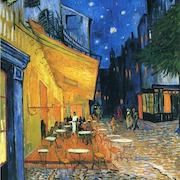
\includegraphics[width=20mm]{figures/cafe_terrace_at_night.png}}{original}
        \\
        \end{tabular}
\caption{ Best Images for Default Parameters}
\normalsize
\end{figure}

\begin{figure}[H]
    \centering
    \begin{tabular}{c c}
        \subf{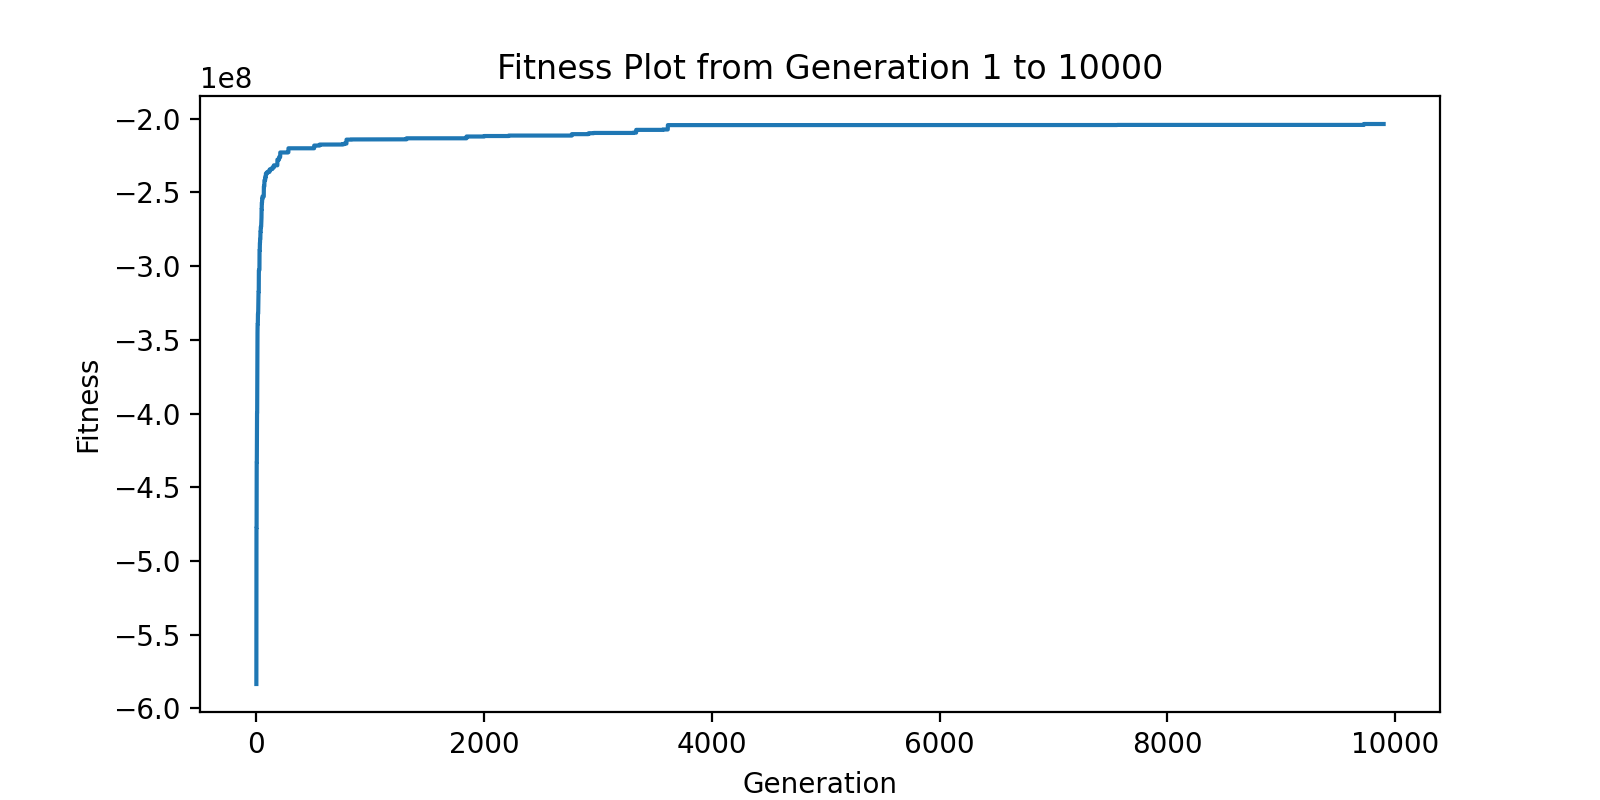
\includegraphics[width=75mm]{figures/def/cafe_terrace_at_night_fitness.png}}{gens 1 to 10000}
        &
        \subf{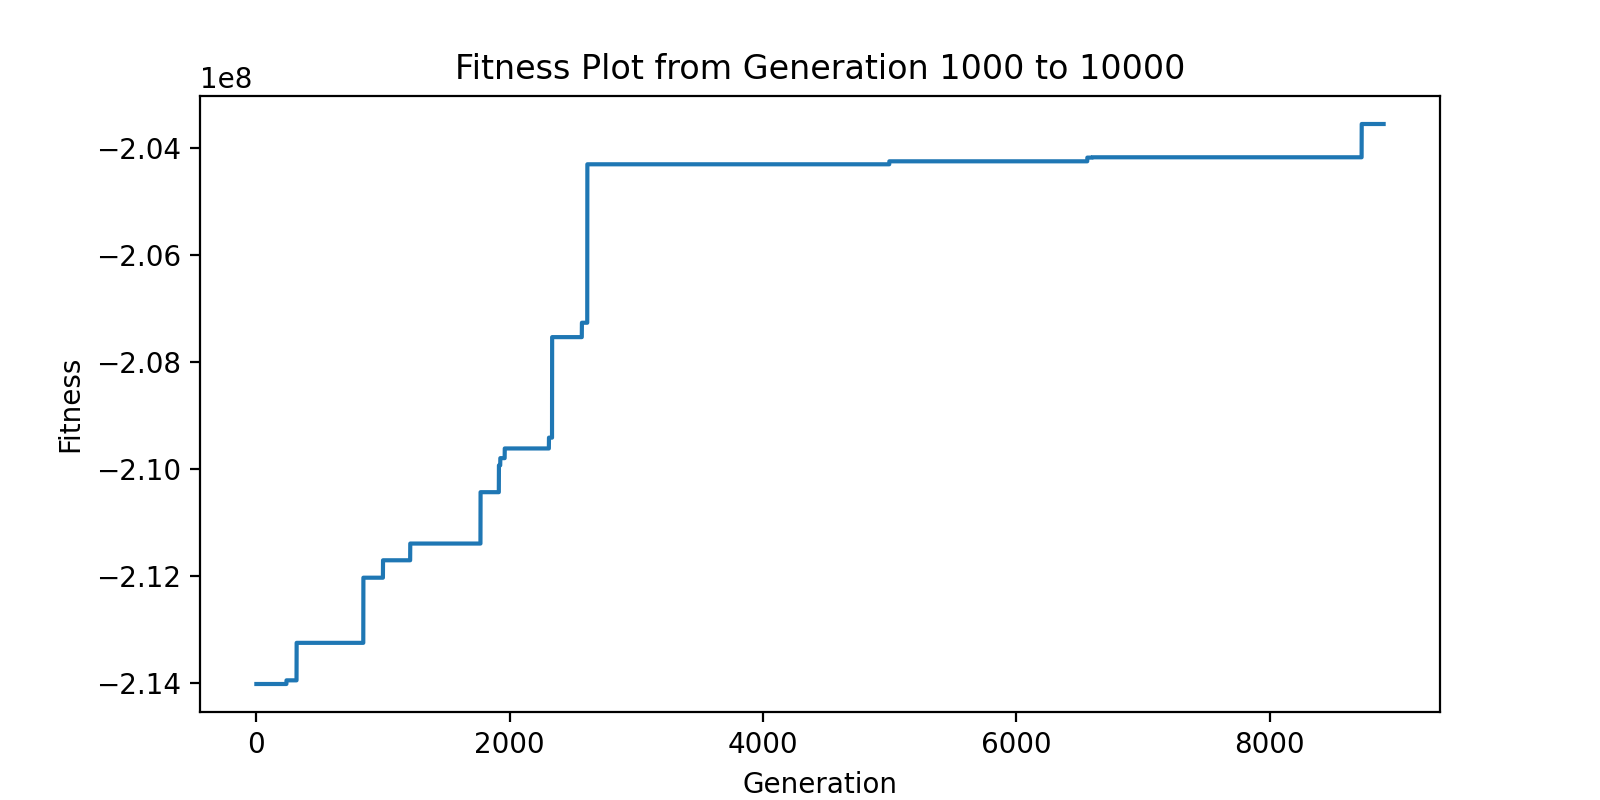
\includegraphics[width=75mm]{figures/def/cafe_terrace_at_night_fitness_1000.png}}{gens 1000 to 10000}
        \\
        \end{tabular}
\caption{ Fitness Plots for Default Parameters}
\normalsize
\end{figure}



\subsection{\textbf{\Large Number of Individuals \(<num\_inds>\)}}

The number of individuals is the size of the population. The individuals are used to generate next generation.
Higher the number of individuals, the more diverse the starting population is.

\subsubsection{\textbf{Number of Individuals  = 5}}

\begin{figure}[H]
    \centering
    \begin{tabular}{c c c c c c}
          \subf{
\includegraphics[width=20mm]{figures/ind-5/cafe_terrace_at_night_gen_0.png}}{gens 0}
        &
        \subf{
\includegraphics[width=20mm]{figures/ind-5/cafe_terrace_at_night_gen_999.png}}{gens 1000}
        &
        \subf{
\includegraphics[width=20mm]{figures/ind-5/cafe_terrace_at_night_gen_1999.png}}{gens 2000}
        &
        \subf{
\includegraphics[width=20mm]{figures/ind-5/cafe_terrace_at_night_gen_2999.png}}{gens 3000}
        &
        \subf{
\includegraphics[width=20mm]{figures/ind-5/cafe_terrace_at_night_gen_3999.png}}{gens 4000}
        &
        \subf{
\includegraphics[width=20mm]{figures/ind-5/cafe_terrace_at_night_gen_4999.png}}{gens 5000}
        \\
        \end{tabular}
    \begin{tabular}{c c c c c c}
        \subf{
\includegraphics[width=20mm]{figures/ind-5/cafe_terrace_at_night_gen_5999.png}}{gens 6000}
        &
        \subf{
\includegraphics[width=20mm]{figures/ind-5/cafe_terrace_at_night_gen_6999.png}}{gens 7000}
        &
        \subf{
\includegraphics[width=20mm]{figures/ind-5/cafe_terrace_at_night_gen_7999.png}}{gens 8000}
        &
        \subf{
\includegraphics[width=20mm]{figures/ind-5/cafe_terrace_at_night_gen_8999.png}}{gens 9000}
        &
        \subf{
\includegraphics[width=20mm]{figures/ind-5/cafe_terrace_at_night_gen_9999.png}}{gens 10000}
        &
        \subf{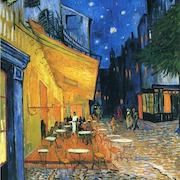
\includegraphics[width=20mm]{figures/cafe_terrace_at_night.png}}{original}
        \\
        \end{tabular}
\caption{ Best Images for $<num\_inds>$ = 5}
\normalsize
\end{figure}

\begin{figure}[H]
    \centering
    \begin{tabular}{c c}
        \subf{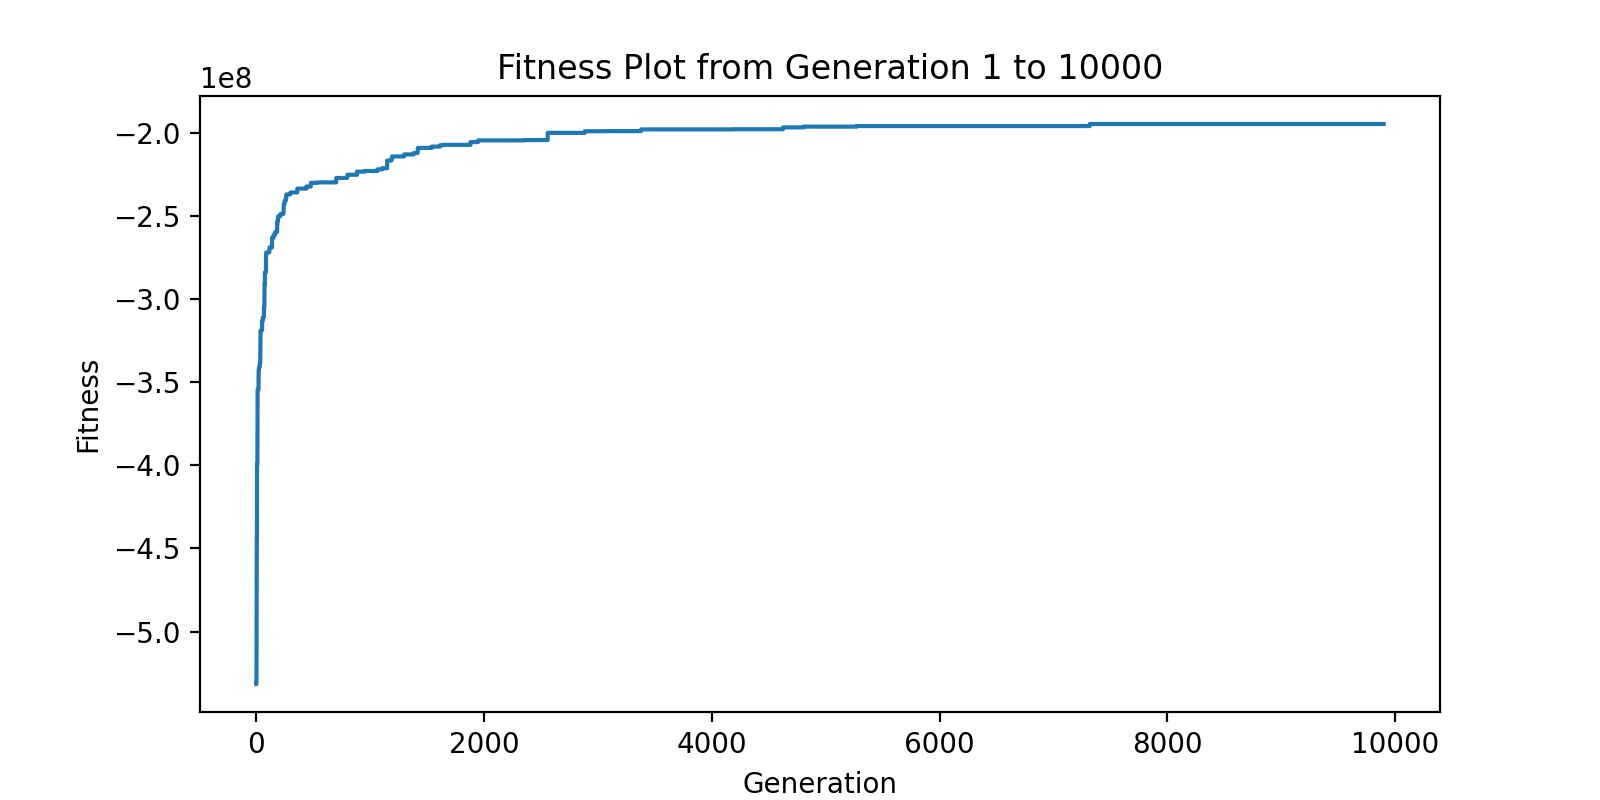
\includegraphics[width=75mm]{figures/ind-5/cafe_terrace_at_night_fitness.png}}{gens 1 to 10000}
        &
        \subf{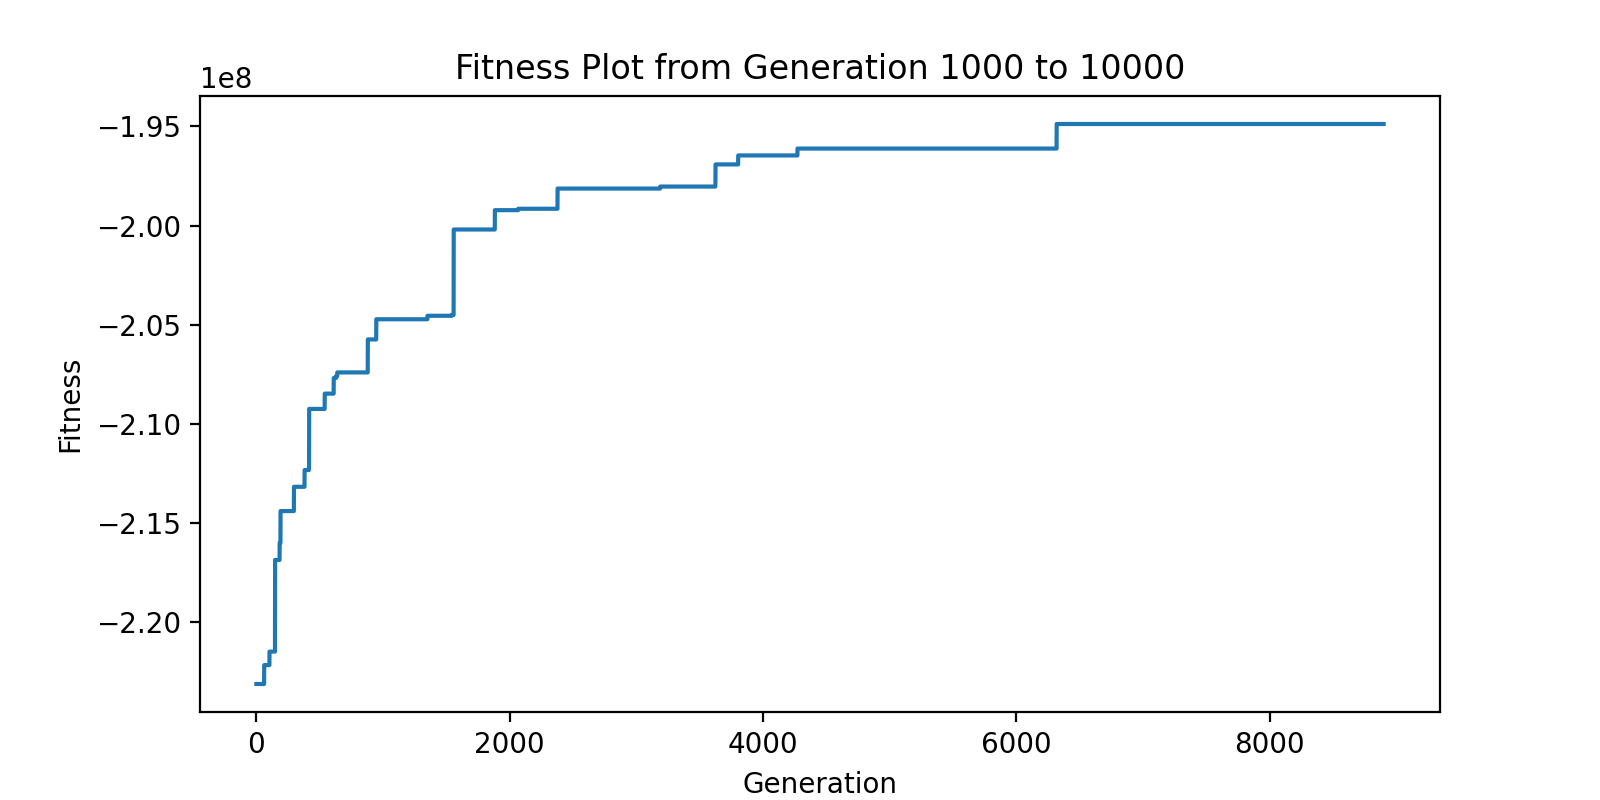
\includegraphics[width=75mm]{figures/ind-5/cafe_terrace_at_night_fitness_1000.png}}{gens 1000 to 10000}
        \\
        \end{tabular}
\caption{ Fitness Plots for $<num\_inds>$ = 5}
\normalsize
\end{figure}

\subsubsection{\textbf{Number of Individuals  = 10}}

\begin{figure}[H]
    \centering
    \begin{tabular}{c c c c c c}
          \subf{
\includegraphics[width=20mm]{figures/ind-10/cafe_terrace_at_night_gen_0.png}}{gens 0}
        &
        \subf{
\includegraphics[width=20mm]{figures/ind-10/cafe_terrace_at_night_gen_999.png}}{gens 1000}
        &
        \subf{
\includegraphics[width=20mm]{figures/ind-10/cafe_terrace_at_night_gen_1999.png}}{gens 2000}
        &
        \subf{
\includegraphics[width=20mm]{figures/ind-10/cafe_terrace_at_night_gen_2999.png}}{gens 3000}
        &
        \subf{
\includegraphics[width=20mm]{figures/ind-10/cafe_terrace_at_night_gen_3999.png}}{gens 4000}
        &
        \subf{
\includegraphics[width=20mm]{figures/ind-10/cafe_terrace_at_night_gen_4999.png}}{gens 5000}
        \\
        \end{tabular}
    \begin{tabular}{c c c c c c}
        \subf{
\includegraphics[width=20mm]{figures/ind-10/cafe_terrace_at_night_gen_5999.png}}{gens 6000}
        &
        \subf{
\includegraphics[width=20mm]{figures/ind-10/cafe_terrace_at_night_gen_6999.png}}{gens 7000}
        &
        \subf{
\includegraphics[width=20mm]{figures/ind-10/cafe_terrace_at_night_gen_7999.png}}{gens 8000}
        &
        \subf{
\includegraphics[width=20mm]{figures/ind-10/cafe_terrace_at_night_gen_8999.png}}{gens 9000}
        &
        \subf{
\includegraphics[width=20mm]{figures/ind-10/cafe_terrace_at_night_gen_9999.png}}{gens 10000}
        &
        \subf{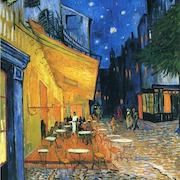
\includegraphics[width=20mm]{figures/cafe_terrace_at_night.png}}{original}
        \\
        \end{tabular}
\caption{ Best Images for $<num\_inds>$ = 10}
\normalsize
\end{figure}

\begin{figure}[H]
    \centering
    \begin{tabular}{c c}
        \subf{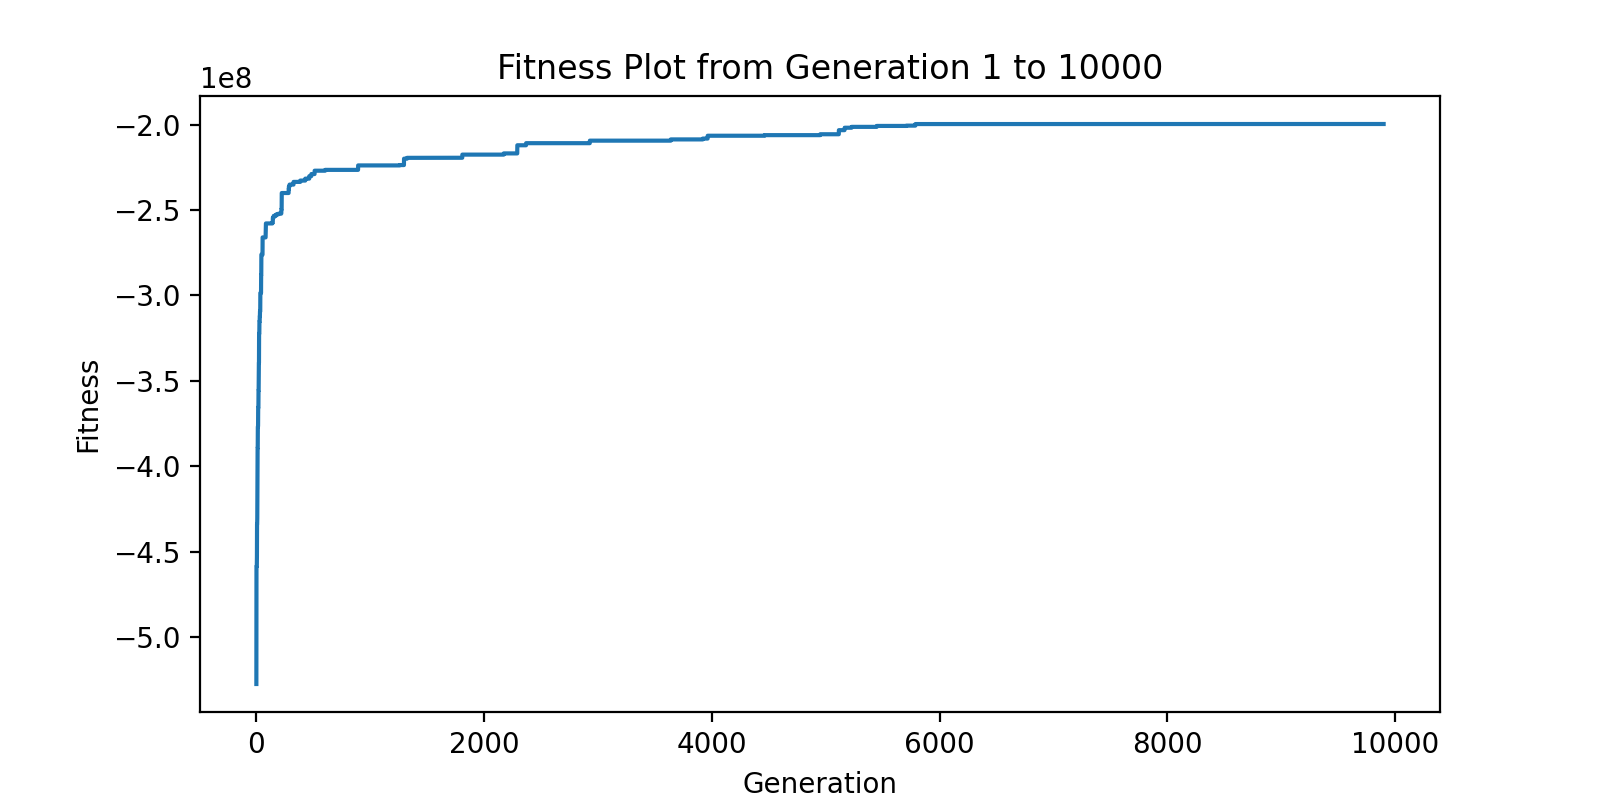
\includegraphics[width=75mm]{figures/ind-10/cafe_terrace_at_night_fitness.png}}{gens 1 to 10000}
        &
        \subf{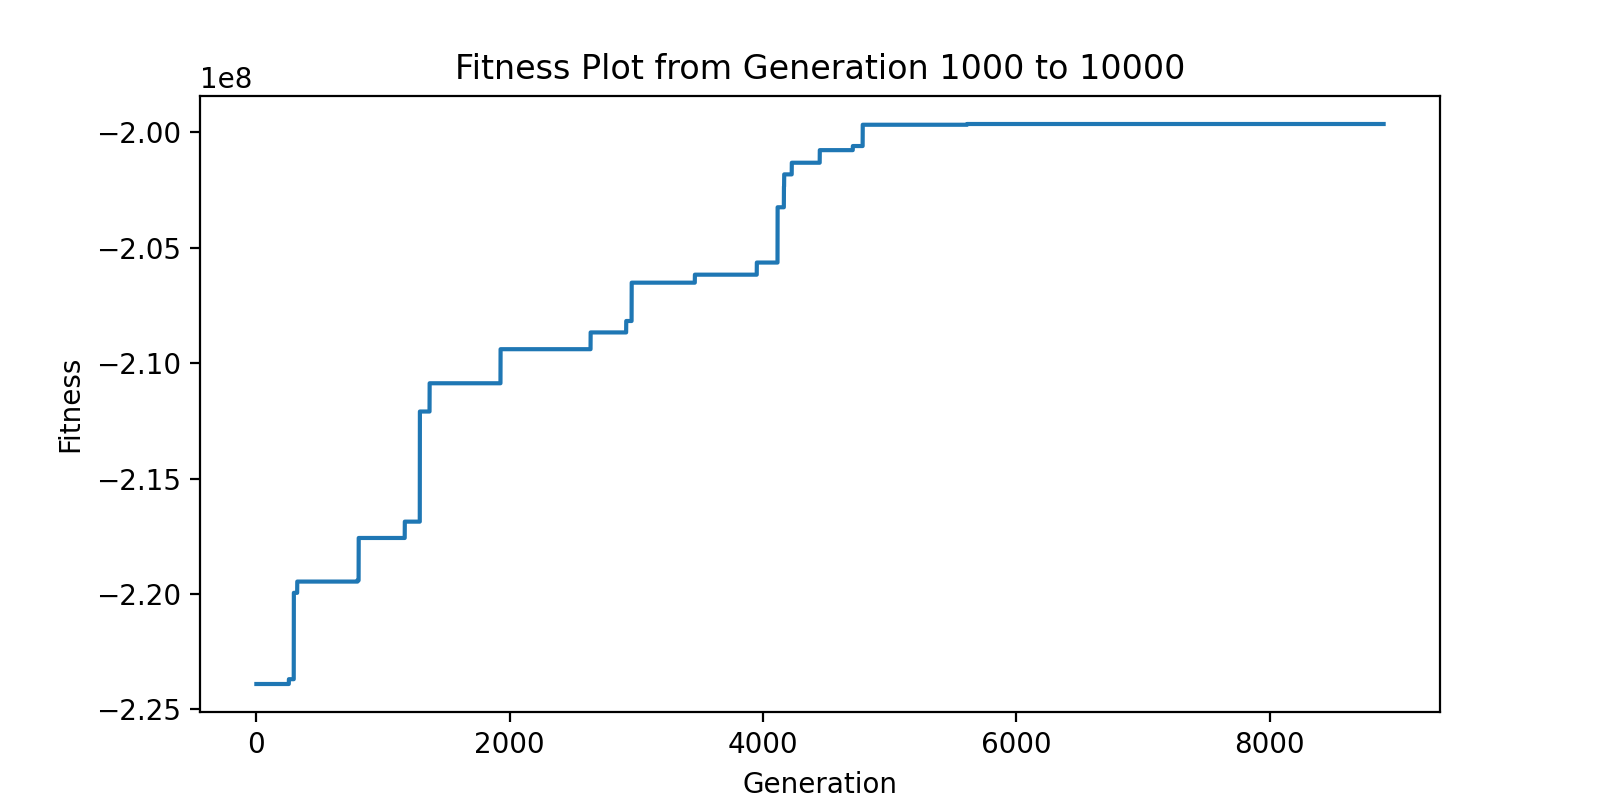
\includegraphics[width=75mm]{figures/ind-10/cafe_terrace_at_night_fitness_1000.png}}{gens 1000 to 10000}
        \\
        \end{tabular}
\caption{ Fitness Plots for $<num\_inds>$ = 10}
\normalsize
\end{figure}

\subsubsection{\textbf{Number of Individuals  = 40}}

\begin{figure}[H]
    \centering
    \begin{tabular}{c c c c c c}
          \subf{
\includegraphics[width=20mm]{figures/ind-40/cafe_terrace_at_night_gen_0.png}}{gens 0}
        &
        \subf{
\includegraphics[width=20mm]{figures/ind-40/cafe_terrace_at_night_gen_999.png}}{gens 1000}
        &
        \subf{
\includegraphics[width=20mm]{figures/ind-40/cafe_terrace_at_night_gen_1999.png}}{gens 2000}
        &
        \subf{
\includegraphics[width=20mm]{figures/ind-40/cafe_terrace_at_night_gen_2999.png}}{gens 3000}
        &
        \subf{
\includegraphics[width=20mm]{figures/ind-40/cafe_terrace_at_night_gen_3999.png}}{gens 4000}
        &
        \subf{
\includegraphics[width=20mm]{figures/ind-40/cafe_terrace_at_night_gen_4999.png}}{gens 5000}
        \\
        \end{tabular}
    \begin{tabular}{c c c c c c}
        \subf{
\includegraphics[width=20mm]{figures/ind-40/cafe_terrace_at_night_gen_5999.png}}{gens 6000}
        &
        \subf{
\includegraphics[width=20mm]{figures/ind-40/cafe_terrace_at_night_gen_6999.png}}{gens 7000}
        &
        \subf{\includegraphics[width=20mm]{figures/ind-40/cafe_terrace_at_night_gen_7999.png}}{gens 8000}
        &
        \subf{\includegraphics[width=20mm]{figures/ind-40/cafe_terrace_at_night_gen_8999.png}}{gens 9000}
        &
        \subf{\includegraphics[width=20mm]{figures/ind-40/cafe_terrace_at_night_gen_9999.png}}{gens 10000}
        &
        \subf{\includegraphics[width=20mm]{figures/cafe_terrace_at_night.png}}{original}
        \\
        \end{tabular}
\caption{ Best Images for $<num\_inds>$ = 40}
\normalsize
\end{figure}

\begin{figure}[H]
    \centering
    \begin{tabular}{c c}
        \subf{\includegraphics[width=75mm]{figures/ind-40/cafe_terrace_at_night_fitness.png}}{gens 1 to 10000}
        &
        \subf{\includegraphics[width=75mm]{figures/ind-40/cafe_terrace_at_night_fitness_1000.png}}{gens 1000 to 10000}
        \\
        \end{tabular}
\caption{ Fitness Plots for $<num\_inds>$ = 40}
\normalsize
\end{figure}

\subsubsection{\textbf{Number of Individuals  = 60}}

\begin{figure}[H]
    \centering
    \begin{tabular}{c c c c c c}
          \subf{\includegraphics[width=20mm]{figures/ind-60/cafe_terrace_at_night_gen_0.png}}{gens 0}
        &
        \subf{\includegraphics[width=20mm]{figures/ind-60/cafe_terrace_at_night_gen_999.png}}{gens 1000}
        &
        \subf{\includegraphics[width=20mm]{figures/ind-60/cafe_terrace_at_night_gen_1999.png}}{gens 2000}
        &
        \subf{\includegraphics[width=20mm]{figures/ind-60/cafe_terrace_at_night_gen_2999.png}}{gens 3000}
        &
        \subf{\includegraphics[width=20mm]{figures/ind-60/cafe_terrace_at_night_gen_3999.png}}{gens 4000}
        &
        \subf{\includegraphics[width=20mm]{figures/ind-60/cafe_terrace_at_night_gen_4999.png}}{gens 5000}
        \\
        \end{tabular}
    \begin{tabular}{c c c c c c}
        \subf{\includegraphics[width=20mm]{figures/ind-60/cafe_terrace_at_night_gen_5999.png}}{gens 6000}
        &
        \subf{\includegraphics[width=20mm]{figures/ind-60/cafe_terrace_at_night_gen_6999.png}}{gens 7000}
        &
        \subf{\includegraphics[width=20mm]{figures/ind-60/cafe_terrace_at_night_gen_7999.png}}{gens 8000}
        &
        \subf{\includegraphics[width=20mm]{figures/ind-60/cafe_terrace_at_night_gen_8999.png}}{gens 9000}
        &
        \subf{\includegraphics[width=20mm]{figures/ind-60/cafe_terrace_at_night_gen_9999.png}}{gens 10000}
        &
        \subf{\includegraphics[width=20mm]{figures/cafe_terrace_at_night.png}}{original}
        \\
        \end{tabular}
\caption{ Best Images for $<num\_inds>$ = 60}
\normalsize
\end{figure}

\begin{figure}[H]
    \centering
    \begin{tabular}{c c}
        \subf{\includegraphics[width=75mm]{figures/ind-60/cafe_terrace_at_night_fitness.png}}{gens 1 to 10000}
        &
        \subf{\includegraphics[width=75mm]{figures/ind-60/cafe_terrace_at_night_fitness_1000.png}}{gens 1000 to 10000}
        \\
        \end{tabular}
\caption{ Fitness Plots for $<num\_inds>$ = 60}
\normalsize
\end{figure}

A larger population size has better chance in exploring the solution space and finding the global optimum.
However, it also means that the algorithm will take more time to converge.
The smaller population size has better advantage in exploitation, that is searching around the promising regions of the solution space.

\medskip


A larger population size helps a faster convergence, that means that the algorithm is able to find the optimal solution in less number of generations, eventhougn the algorithm takes more processing power.
\medskip

Solution quality is also affected by the population size, we can see from the examples that the fitness plots of the larger population size is more smooth and predictable.

\subsection{\textbf{\Large Number of Genes \(<num\_genes>\)}}
Gene size is the number of circles that are used to generate the image. The more circles there are, the more detailed the image is. 
The higher computational cost and harder the problem becomes when the number of genes increases.
\subsubsection{\textbf{Number of Genes  = 15}}
\begin{figure}[H]
    \centering
    \begin{tabular}{c c c c c c}
          \subf{\includegraphics[width=20mm]{figures/genes-15/cafe_terrace_at_night_gen_0.png}}{gens 0}
        &
        \subf{\includegraphics[width=20mm]{figures/genes-15/cafe_terrace_at_night_gen_999.png}}{gens 1000}
        &
        \subf{\includegraphics[width=20mm]{figures/genes-15/cafe_terrace_at_night_gen_1999.png}}{gens 2000}
        &
        \subf{\includegraphics[width=20mm]{figures/genes-15/cafe_terrace_at_night_gen_2999.png}}{gens 3000}
        &
        \subf{\includegraphics[width=20mm]{figures/genes-15/cafe_terrace_at_night_gen_3999.png}}{gens 4000}
        &
        \subf{\includegraphics[width=20mm]{figures/genes-15/cafe_terrace_at_night_gen_4999.png}}{gens 5000}
        \\
        \end{tabular}
    \begin{tabular}{c c c c c c}
        \subf{\includegraphics[width=20mm]{figures/genes-15/cafe_terrace_at_night_gen_5999.png}}{gens 6000}
        &
        \subf{\includegraphics[width=20mm]{figures/genes-15/cafe_terrace_at_night_gen_6999.png}}{gens 7000}
        &
        \subf{\includegraphics[width=20mm]{figures/genes-15/cafe_terrace_at_night_gen_7999.png}}{gens 8000}
        &
        \subf{\includegraphics[width=20mm]{figures/genes-15/cafe_terrace_at_night_gen_8999.png}}{gens 9000}
        &
        \subf{\includegraphics[width=20mm]{figures/genes-15/cafe_terrace_at_night_gen_9999.png}}{gens 10000}
        &
        \subf{\includegraphics[width=20mm]{figures/cafe_terrace_at_night.png}}{original}
        \\
        \end{tabular}
\caption{ Best Images for $<num\_genes>$ = 15}
\normalsize
\end{figure}
\begin{figure}[H]
    \centering
    \begin{tabular}{c c}
        \subf{\includegraphics[width=75mm]{figures/genes-15/cafe_terrace_at_night_fitness.png}}{gens 1 to 10000}
        &
        \subf{\includegraphics[width=75mm]{figures/genes-15/cafe_terrace_at_night_fitness_1000.png}}{gens 1000 to 10000}
        \\
        \end{tabular}
\caption{ Fitness Plots for $<num\_genes>$ = 15}
\normalsize
\end{figure}

\subsubsection{\textbf{Number of Genes  = 30}}
\begin{figure}[H]
    \centering
    \begin{tabular}{c c c c c c}
          \subf{\includegraphics[width=20mm]{figures/genes-30/cafe_terrace_at_night_gen_0.png}}{gens 0}
        &
        \subf{\includegraphics[width=20mm]{figures/genes-30/cafe_terrace_at_night_gen_999.png}}{gens 1000}
        &
        \subf{\includegraphics[width=20mm]{figures/genes-30/cafe_terrace_at_night_gen_1999.png}}{gens 2000}
        &
        \subf{\includegraphics[width=20mm]{figures/genes-30/cafe_terrace_at_night_gen_2999.png}}{gens 3000}
        &
        \subf{\includegraphics[width=20mm]{figures/genes-30/cafe_terrace_at_night_gen_3999.png}}{gens 4000}
        &
        \subf{\includegraphics[width=20mm]{figures/genes-30/cafe_terrace_at_night_gen_4999.png}}{gens 5000}
        \\
        \end{tabular}
    \begin{tabular}{c c c c c c}
        \subf{\includegraphics[width=20mm]{figures/genes-30/cafe_terrace_at_night_gen_5999.png}}{gens 6000}
        &
        \subf{\includegraphics[width=20mm]{figures/genes-30/cafe_terrace_at_night_gen_6999.png}}{gens 7000}
        &
        \subf{\includegraphics[width=20mm]{figures/genes-30/cafe_terrace_at_night_gen_7999.png}}{gens 8000}
        &
        \subf{\includegraphics[width=20mm]{figures/genes-30/cafe_terrace_at_night_gen_8999.png}}{gens 9000}
        &
        \subf{\includegraphics[width=20mm]{figures/genes-30/cafe_terrace_at_night_gen_9999.png}}{gens 10000}
        &
        \subf{\includegraphics[width=20mm]{figures/cafe_terrace_at_night.png}}{original}
        \\
        \end{tabular}
\caption{ Best Images for $<num\_genes>$ = 30}
\normalsize
\end{figure}

\begin{figure}[H]
    \centering
    \begin{tabular}{c c}
        \subf{\includegraphics[width=75mm]{figures/genes-30/cafe_terrace_at_night_fitness.png}}{gens 1 to 10000}
        &
        \subf{\includegraphics[width=75mm]{figures/genes-30/cafe_terrace_at_night_fitness_1000.png}}{gens 1000 to 10000}
        \\
        \end{tabular}
\caption{ Fitness Plots for $<num\_genes>$ = 30}
\normalsize
\end{figure}

\subsubsection{\textbf{Number of Genes  = 80}}
\begin{figure}[H]
    \centering
    \begin{tabular}{c c c c c c}
          \subf{\includegraphics[width=20mm]{figures/genes-80/cafe_terrace_at_night_gen_0.png}}{gens 0}
        &
        \subf{\includegraphics[width=20mm]{figures/genes-80/cafe_terrace_at_night_gen_999.png}}{gens 1000}
        &
        \subf{\includegraphics[width=20mm]{figures/genes-80/cafe_terrace_at_night_gen_1999.png}}{gens 2000}
        &
        \subf{\includegraphics[width=20mm]{figures/genes-80/cafe_terrace_at_night_gen_2999.png}}{gens 3000}
        &
        \subf{\includegraphics[width=20mm]{figures/genes-80/cafe_terrace_at_night_gen_3999.png}}{gens 4000}
        &
        \subf{\includegraphics[width=20mm]{figures/genes-80/cafe_terrace_at_night_gen_4999.png}}{gens 5000}
        \\
        \end{tabular}
    \begin{tabular}{c c c c c c}
        \subf{\includegraphics[width=20mm]{figures/genes-80/cafe_terrace_at_night_gen_5999.png}}{gens 6000}
        &
        \subf{\includegraphics[width=20mm]{figures/genes-80/cafe_terrace_at_night_gen_6999.png}}{gens 7000}
        &
        \subf{\includegraphics[width=20mm]{figures/genes-80/cafe_terrace_at_night_gen_7999.png}}{gens 8000}
        &
        \subf{\includegraphics[width=20mm]{figures/genes-80/cafe_terrace_at_night_gen_8999.png}}{gens 9000}
        &
        \subf{\includegraphics[width=20mm]{figures/genes-80/cafe_terrace_at_night_gen_9999.png}}{gens 10000}
        &
        \subf{\includegraphics[width=20mm]{figures/cafe_terrace_at_night.png}}{original}
        \\
        \end{tabular}
\caption{ Best Images for $<num\_genes>$ = 80}
\normalsize
\end{figure}

\begin{figure}[H]
    \centering
    \begin{tabular}{c c}
        \subf{\includegraphics[width=75mm]{figures/genes-80/cafe_terrace_at_night_fitness.png}}{gens 1 to 10000}
        &
        \subf{\includegraphics[width=75mm]{figures/genes-80/cafe_terrace_at_night_fitness_1000.png}}{gens 1000 to 10000}
        \\
        \end{tabular}
\caption{ Fitness Plots for $<num\_genes>$ = 80}
\normalsize
\end{figure}

\subsubsection{\textbf{Number of Genes  = 120}}
\begin{figure}[H]
    \centering
    \begin{tabular}{c c c c c c}
          \subf{\includegraphics[width=20mm]{figures/genes-120/cafe_terrace_at_night_gen_0.png}}{gens 0}
        &
        \subf{\includegraphics[width=20mm]{figures/genes-120/cafe_terrace_at_night_gen_999.png}}{gens 1000}
        &
        \subf{\includegraphics[width=20mm]{figures/genes-120/cafe_terrace_at_night_gen_1999.png}}{gens 2000}
        &
        \subf{\includegraphics[width=20mm]{figures/genes-120/cafe_terrace_at_night_gen_2999.png}}{gens 3000}
        &
        \subf{\includegraphics[width=20mm]{figures/genes-120/cafe_terrace_at_night_gen_3999.png}}{gens 4000}
        &
        \subf{\includegraphics[width=20mm]{figures/genes-120/cafe_terrace_at_night_gen_4999.png}}{gens 5000}
        \\
        \end{tabular}
    \begin{tabular}{c c c c c c}
        \subf{\includegraphics[width=20mm]{figures/genes-120/cafe_terrace_at_night_gen_5999.png}}{gens 6000}
        &
        \subf{\includegraphics[width=20mm]{figures/genes-120/cafe_terrace_at_night_gen_6999.png}}{gens 7000}
        &
        \subf{\includegraphics[width=20mm]{figures/genes-120/cafe_terrace_at_night_gen_7999.png}}{gens 8000}
        &
        \subf{\includegraphics[width=20mm]{figures/genes-120/cafe_terrace_at_night_gen_8999.png}}{gens 9000}
        &
        \subf{\includegraphics[width=20mm]{figures/genes-120/cafe_terrace_at_night_gen_9999.png}}{gens 10000}
        &
        \subf{\includegraphics[width=20mm]{figures/cafe_terrace_at_night.png}}{original}
        \\
        \end{tabular}
\caption{ Best Images for $<num\_genes>$ = 120}
\normalsize
\end{figure}

\begin{figure}[H]
    \centering
    \begin{tabular}{c c}
        \subf{\includegraphics[width=75mm]{figures/genes-120/cafe_terrace_at_night_fitness.png}}{gens 1 to 10000}
        &
        \subf{\includegraphics[width=75mm]{figures/genes-120/cafe_terrace_at_night_fitness_1000.png}}{gens 1000 to 10000}
        \\
        \end{tabular}
\caption{ Fitness Plots for $<num\_genes>$ = 120}
\normalsize
\end{figure}

For very low number of genes, the algorithm is not able to generate the image properly.
As the number of genes increases, with increased computational cost, the algorithm is able to generate the image with better fitness.
The best fitness is achieved with 120 genes.


\subsection{\Large \textbf{Tournament Size \(<tm\_size>\)}}
\normalsize

Tournament size is the number of individuals that are selected for the tournament. The higher the tournament size, the higher the probability of selecting the best individual for the tournament.


\subsubsection{\textbf{Tournament Size = 2}}
\begin{figure}[H]
    \centering
    \begin{tabular}{c c c c c c}
          \subf{\includegraphics[width=20mm]{figures/tm-2/cafe_terrace_at_night_gen_0.png}}{gens 0}
        &
        \subf{\includegraphics[width=20mm]{figures/tm-2/cafe_terrace_at_night_gen_999.png}}{gens 1000}
        &
        \subf{\includegraphics[width=20mm]{figures/tm-2/cafe_terrace_at_night_gen_1999.png}}{gens 2000}
        &
        \subf{\includegraphics[width=20mm]{figures/tm-2/cafe_terrace_at_night_gen_2999.png}}{gens 3000}
        &
        \subf{\includegraphics[width=20mm]{figures/tm-2/cafe_terrace_at_night_gen_3999.png}}{gens 4000}
        &
        \subf{\includegraphics[width=20mm]{figures/tm-2/cafe_terrace_at_night_gen_4999.png}}{gens 5000}
        \\
        \end{tabular}
    \begin{tabular}{c c c c c c}
        \subf{\includegraphics[width=20mm]{figures/tm-2/cafe_terrace_at_night_gen_5999.png}}{gens 6000}
        &
        \subf{\includegraphics[width=20mm]{figures/tm-2/cafe_terrace_at_night_gen_6999.png}}{gens 7000}
        &
        \subf{\includegraphics[width=20mm]{figures/tm-2/cafe_terrace_at_night_gen_7999.png}}{gens 8000}
        &
        \subf{\includegraphics[width=20mm]{figures/tm-2/cafe_terrace_at_night_gen_8999.png}}{gens 9000}
        &
        \subf{\includegraphics[width=20mm]{figures/tm-2/cafe_terrace_at_night_gen_9999.png}}{gens 10000}
        &
        \subf{\includegraphics[width=20mm]{figures/cafe_terrace_at_night.png}}{original}
        \\
        \end{tabular}
\caption{ Best Images for $<tm\_size>$ = 2}
\normalsize
\end{figure}

\begin{figure}[H]
    \centering
    \begin{tabular}{c c}
        \subf{\includegraphics[width=75mm]{figures/tm-2/cafe_terrace_at_night_fitness.png}}{gens 1 to 10000}
        &
        \subf{\includegraphics[width=75mm]{figures/tm-2/cafe_terrace_at_night_fitness_1000.png}}{gens 1000 to 10000}
        \\
        \end{tabular}
\caption{ Fitness Plots for $<tm\_size>$ = 2}
\normalsize
\end{figure}

\subsubsection{\textbf{Tournament Size = 8}}
\begin{figure}[H]
    \centering
    \begin{tabular}{c c c c c c}
          \subf{\includegraphics[width=20mm]{figures/tm-8/cafe_terrace_at_night_gen_0.png}}{gens 0}
        &
        \subf{\includegraphics[width=20mm]{figures/tm-8/cafe_terrace_at_night_gen_999.png}}{gens 1000}
        &
        \subf{\includegraphics[width=20mm]{figures/tm-8/cafe_terrace_at_night_gen_1999.png}}{gens 2000}
        &
        \subf{\includegraphics[width=20mm]{figures/tm-8/cafe_terrace_at_night_gen_2999.png}}{gens 3000}
        &
        \subf{\includegraphics[width=20mm]{figures/tm-8/cafe_terrace_at_night_gen_3999.png}}{gens 4000}
        &
        \subf{\includegraphics[width=20mm]{figures/tm-8/cafe_terrace_at_night_gen_4999.png}}{gens 5000}
        \\
        \end{tabular}
    \begin{tabular}{c c c c c c}
        \subf{\includegraphics[width=20mm]{figures/tm-8/cafe_terrace_at_night_gen_5999.png}}{gens 6000}
        &
        \subf{\includegraphics[width=20mm]{figures/tm-8/cafe_terrace_at_night_gen_6999.png}}{gens 7000}
        &
        \subf{\includegraphics[width=20mm]{figures/tm-8/cafe_terrace_at_night_gen_7999.png}}{gens 8000}
        &
        \subf{\includegraphics[width=20mm]{figures/tm-8/cafe_terrace_at_night_gen_8999.png}}{gens 9000}
        &
        \subf{\includegraphics[width=20mm]{figures/tm-8/cafe_terrace_at_night_gen_9999.png}}{gens 10000}
        &
        \subf{\includegraphics[width=20mm]{figures/cafe_terrace_at_night.png}}{original}
        \\
        \end{tabular}
\caption{ Best Images for $<tm\_size>$ = 8}
\normalsize
\end{figure}
\vspace{-0.5cm}
\begin{figure}[H]
    \centering
    \begin{tabular}{c c}
        \subf{\includegraphics[width=75mm]{figures/tm-8/cafe_terrace_at_night_fitness.png}}{gens 1 to 10000}
        &
        \subf{\includegraphics[width=75mm]{figures/tm-8/cafe_terrace_at_night_fitness_1000.png}}{gens 1000 to 10000}
        \\
        \end{tabular}
\caption{ Fitness Plots for $<tm\_size>$ = 8}
\normalsize
\end{figure}
\vspace{-0.5cm}
\subsubsection{\textbf{Tournament Size = 16}}
\begin{figure}[H]
    \centering
    \begin{tabular}{c c c c c c}
          \subf{\includegraphics[width=20mm]{figures/tm-16/cafe_terrace_at_night_gen_0.png}}{gens 0}
        &
        \subf{\includegraphics[width=20mm]{figures/tm-16/cafe_terrace_at_night_gen_999.png}}{gens 1000}
        &
        \subf{\includegraphics[width=20mm]{figures/tm-16/cafe_terrace_at_night_gen_1999.png}}{gens 2000}
        &
        \subf{\includegraphics[width=20mm]{figures/tm-16/cafe_terrace_at_night_gen_2999.png}}{gens 3000}
        &
        \subf{\includegraphics[width=20mm]{figures/tm-16/cafe_terrace_at_night_gen_3999.png}}{gens 4000}
        &
        \subf{\includegraphics[width=20mm]{figures/tm-16/cafe_terrace_at_night_gen_4999.png}}{gens 5000}
        \\
        \end{tabular}
    \begin{tabular}{c c c c c c}
        \subf{\includegraphics[width=20mm]{figures/tm-16/cafe_terrace_at_night_gen_5999.png}}{gens 6000}
        &
        \subf{\includegraphics[width=20mm]{figures/tm-16/cafe_terrace_at_night_gen_6999.png}}{gens 7000}
        &
        \subf{\includegraphics[width=20mm]{figures/tm-16/cafe_terrace_at_night_gen_7999.png}}{gens 8000}
        &
        \subf{\includegraphics[width=20mm]{figures/tm-16/cafe_terrace_at_night_gen_8999.png}}{gens 9000}
        &
        \subf{\includegraphics[width=20mm]{figures/tm-16/cafe_terrace_at_night_gen_9999.png}}{gens 10000}
        &
        \subf{\includegraphics[width=20mm]{figures/cafe_terrace_at_night.png}}{original}
        \\
        \end{tabular}
\caption{ Best Images for $<tm\_size>$ = 16}
\normalsize
\end{figure}

\begin{figure}[H]
    \centering
    \begin{tabular}{c c}
        \subf{\includegraphics[width=75mm]{figures/tm-16/cafe_terrace_at_night_fitness.png}}{gens 1 to 10000}
        &
        \subf{\includegraphics[width=75mm]{figures/tm-16/cafe_terrace_at_night_fitness_1000.png}}{gens 1000 to 10000}
        \\
        \end{tabular}
\caption{ Fitness Plots for $<tm\_size>$ = 16}
\normalsize
\end{figure}


The results seem similar, and the results are highly dependent on the random seed.

\medskip

What can be deducted is the tournament size 2 is favored by the exploitation and finds a good enough solution around a minimum.
The tournament size 16 is favored by the exploration and finds a better solution around the global minimum but it takes a lot more effort.
The inbetween tournament size 8, which performs very similar to size 5,  is a good compromise between the two.

\subsection{\Large \textbf{Fraction of Elites \(<frac\_elites>\)}}
Elites are very effective in keeping the population fit, since they are directly copied to the next generation.
The fraction of elites is the percentage of the population that is copied to the next generation.
The elites are also included in the reproduction process, so they can be mutated and crossed over.
This approach gives more chance to the elites to be replaced by better individuals.
% \vspace{-0.5cm}
\subsubsection{\textbf{Fraction of Elites = 0.04}}
\begin{figure}[H]
    \centering
    \begin{tabular}{c c c c c c}
          \subf{\includegraphics[width=20mm]{figures/elites-0.04/cafe_terrace_at_night_gen_0.png}}{gens 0}
        &
        \subf{\includegraphics[width=20mm]{figures/elites-0.04/cafe_terrace_at_night_gen_999.png}}{gens 1000}
        &
        \subf{\includegraphics[width=20mm]{figures/elites-0.04/cafe_terrace_at_night_gen_1999.png}}{gens 2000}
        &
        \subf{\includegraphics[width=20mm]{figures/elites-0.04/cafe_terrace_at_night_gen_2999.png}}{gens 3000}
        &
        \subf{\includegraphics[width=20mm]{figures/elites-0.04/cafe_terrace_at_night_gen_3999.png}}{gens 4000}
        &
        \subf{\includegraphics[width=20mm]{figures/elites-0.04/cafe_terrace_at_night_gen_4999.png}}{gens 5000}
        \\
        \end{tabular}
    \begin{tabular}{c c c c c c}
        \subf{\includegraphics[width=20mm]{figures/elites-0.04/cafe_terrace_at_night_gen_5999.png}}{gens 6000}
        &
        \subf{\includegraphics[width=20mm]{figures/elites-0.04/cafe_terrace_at_night_gen_6999.png}}{gens 7000}
        &
        \subf{\includegraphics[width=20mm]{figures/elites-0.04/cafe_terrace_at_night_gen_7999.png}}{gens 8000}
        &
        \subf{\includegraphics[width=20mm]{figures/elites-0.04/cafe_terrace_at_night_gen_8999.png}}{gens 9000}
        &
        \subf{\includegraphics[width=20mm]{figures/elites-0.04/cafe_terrace_at_night_gen_9999.png}}{gens 10000}
        &
        \subf{\includegraphics[width=20mm]{figures/cafe_terrace_at_night.png}}{original}
        \\
        \end{tabular}
\caption{ Best Images for $<frac\_elites>$ = 0.04}
\normalsize
\end{figure}
\vspace{-0.5cm}
\begin{figure}[H]
    \centering
    \begin{tabular}{c c}
        \subf{\includegraphics[width=75mm]{figures/elites-0.04/cafe_terrace_at_night_fitness.png}}{gens 1 to 10000}
        &
        \subf{\includegraphics[width=75mm]{figures/elites-0.04/cafe_terrace_at_night_fitness_1000.png}}{gens 1000 to 10000}
        \\
        \end{tabular}
\caption{ Fitness Plots for $<frac\_elites>$ = 0.04}
\normalsize
\end{figure}
\vspace{-0.5cm}
\subsubsection{\textbf{Fraction of Elites = 0.35}}
\begin{figure}[H]
    \centering
    \begin{tabular}{c c c c c c}
          \subf{\includegraphics[width=20mm]{figures/elites-0.35/cafe_terrace_at_night_gen_0.png}}{gens 0}
        &
        \subf{\includegraphics[width=20mm]{figures/elites-0.35/cafe_terrace_at_night_gen_999.png}}{gens 1000}
        &
        \subf{\includegraphics[width=20mm]{figures/elites-0.35/cafe_terrace_at_night_gen_1999.png}}{gens 2000}
        &
        \subf{\includegraphics[width=20mm]{figures/elites-0.35/cafe_terrace_at_night_gen_2999.png}}{gens 3000}
        &
        \subf{\includegraphics[width=20mm]{figures/elites-0.35/cafe_terrace_at_night_gen_3999.png}}{gens 4000}
        &
        \subf{\includegraphics[width=20mm]{figures/elites-0.35/cafe_terrace_at_night_gen_4999.png}}{gens 5000}
        \\
        \end{tabular}
    \begin{tabular}{c c c c c c}
        \subf{\includegraphics[width=20mm]{figures/elites-0.35/cafe_terrace_at_night_gen_5999.png}}{gens 6000}
        &
        \subf{\includegraphics[width=20mm]{figures/elites-0.35/cafe_terrace_at_night_gen_6999.png}}{gens 7000}
        &
        \subf{\includegraphics[width=20mm]{figures/elites-0.35/cafe_terrace_at_night_gen_7999.png}}{gens 8000}
        &
        \subf{\includegraphics[width=20mm]{figures/elites-0.35/cafe_terrace_at_night_gen_8999.png}}{gens 9000}
        &
        \subf{\includegraphics[width=20mm]{figures/elites-0.35/cafe_terrace_at_night_gen_9999.png}}{gens 10000}
        &
        \subf{\includegraphics[width=20mm]{figures/cafe_terrace_at_night.png}}{original}
        \\
        \end{tabular}
\caption{ Best Images for $<frac\_elites>$ = 0.35}
\normalsize
\end{figure}

\begin{figure}[H]
    \centering
    \begin{tabular}{c c}
        \subf{\includegraphics[width=75mm]{figures/elites-0.35/cafe_terrace_at_night_fitness.png}}{gens 1 to 10000}
        &
        \subf{\includegraphics[width=75mm]{figures/elites-0.35/cafe_terrace_at_night_fitness_1000.png}}{gens 1000 to 10000}
        \\
        \end{tabular}
\caption{ Fitness Plots for $<frac\_elites>$ = 0.35}
\normalsize
\end{figure}
\vspace{-0.5cm}
The most important aspect of the elites are the preservation of the best individuals.
The first case is where elite number is zero. It can be seen that the random chance factor is high and the fitness plot is blocky.
The second case is the default case, where the elites are 20\% of the population. It is better than the first case, but the fitness plot is still discrete.
The third case is where the every 1/3rd individual is an elite. The fitness plot is smooth and the best individual is better than the previous cases.

\subsection{\Large \textbf{Fraction of Parents \(<frac\_parents>\)}}
The number of parents is the number of individuals that are selected for reproduction.
The genetic reproduction is done by crossing over the genes of the parents.
The elites are also included in the reproduction process.
% \vspace{-0.5cm}
\subsubsection{\textbf{Fraction of Parents = 0.15}}
\begin{figure}[H]
    \centering
    \begin{tabular}{c c c c c c}
          \subf{\includegraphics[width=20mm]{figures/parents-0.15/cafe_terrace_at_night_gen_0.png}}{gens 0}
        &
        \subf{\includegraphics[width=20mm]{figures/parents-0.15/cafe_terrace_at_night_gen_999.png}}{gens 1000}
        &
        \subf{\includegraphics[width=20mm]{figures/parents-0.15/cafe_terrace_at_night_gen_1999.png}}{gens 2000}
        &
        \subf{\includegraphics[width=20mm]{figures/parents-0.15/cafe_terrace_at_night_gen_2999.png}}{gens 3000}
        &
        \subf{\includegraphics[width=20mm]{figures/parents-0.15/cafe_terrace_at_night_gen_3999.png}}{gens 4000}
        &
        \subf{\includegraphics[width=20mm]{figures/parents-0.15/cafe_terrace_at_night_gen_4999.png}}{gens 5000}
        \\
        \end{tabular}
    \begin{tabular}{c c c c c c}
        \subf{\includegraphics[width=20mm]{figures/parents-0.15/cafe_terrace_at_night_gen_5999.png}}{gens 6000}
        &
        \subf{\includegraphics[width=20mm]{figures/parents-0.15/cafe_terrace_at_night_gen_6999.png}}{gens 7000}
        &
        \subf{\includegraphics[width=20mm]{figures/parents-0.15/cafe_terrace_at_night_gen_7999.png}}{gens 8000}
        &
        \subf{\includegraphics[width=20mm]{figures/parents-0.15/cafe_terrace_at_night_gen_8999.png}}{gens 9000}
        &
        \subf{\includegraphics[width=20mm]{figures/parents-0.15/cafe_terrace_at_night_gen_9999.png}}{gens 10000}
        &
        \subf{\includegraphics[width=20mm]{figures/cafe_terrace_at_night.png}}{original}
        \\
        \end{tabular}
\caption{ Best Images for $<frac\_parents>$ = 0.15}
\normalsize
\end{figure}
\vspace{-0.5cm}
\begin{figure}[H]
    \centering
    \begin{tabular}{c c}
        \subf{\includegraphics[width=75mm]{figures/parents-0.15/cafe_terrace_at_night_fitness.png}}{gens 1 to 10000}
        &
        \subf{\includegraphics[width=75mm]{figures/parents-0.15/cafe_terrace_at_night_fitness_1000.png}}{gens 1000 to 10000}
        \\
        \end{tabular}
\caption{ Fitness Plots for $<frac\_parents>$ = 0.15}
\normalsize
\end{figure}


\subsubsection{\textbf{Fraction of Parents = 0.3}}
\begin{figure}[H]
    \centering
    \begin{tabular}{c c c c c c}
          \subf{\includegraphics[width=20mm]{figures/parents-0.3/cafe_terrace_at_night_gen_0.png}}{gens 0}
        &
        \subf{\includegraphics[width=20mm]{figures/parents-0.3/cafe_terrace_at_night_gen_999.png}}{gens 1000}
        &
        \subf{\includegraphics[width=20mm]{figures/parents-0.3/cafe_terrace_at_night_gen_1999.png}}{gens 2000}
        &
        \subf{\includegraphics[width=20mm]{figures/parents-0.3/cafe_terrace_at_night_gen_2999.png}}{gens 3000}
        &
        \subf{\includegraphics[width=20mm]{figures/parents-0.3/cafe_terrace_at_night_gen_3999.png}}{gens 4000}
        &
        \subf{\includegraphics[width=20mm]{figures/parents-0.3/cafe_terrace_at_night_gen_4999.png}}{gens 5000}
        \\
        \end{tabular}
    \begin{tabular}{c c c c c c}
        \subf{\includegraphics[width=20mm]{figures/parents-0.3/cafe_terrace_at_night_gen_5999.png}}{gens 6000}
        &
        \subf{\includegraphics[width=20mm]{figures/parents-0.3/cafe_terrace_at_night_gen_6999.png}}{gens 7000}
        &
        \subf{\includegraphics[width=20mm]{figures/parents-0.3/cafe_terrace_at_night_gen_7999.png}}{gens 8000}
        &
        \subf{\includegraphics[width=20mm]{figures/parents-0.3/cafe_terrace_at_night_gen_8999.png}}{gens 9000}
        &
        \subf{\includegraphics[width=20mm]{figures/parents-0.3/cafe_terrace_at_night_gen_9999.png}}{gens 10000}
        &
        \subf{\includegraphics[width=20mm]{figures/cafe_terrace_at_night.png}}{original}
        \\
        \end{tabular}
\caption{ Best Images for $<frac\_parents>$ = 0.3}
\normalsize
\end{figure}

\begin{figure}[H]
    \centering
    \begin{tabular}{c c}
        \subf{\includegraphics[width=75mm]{figures/parents-0.3/cafe_terrace_at_night_fitness.png}}{gens 1 to 10000}
        &
        \subf{\includegraphics[width=75mm]{figures/parents-0.3/cafe_terrace_at_night_fitness_1000.png}}{gens 1000 to 10000}
        \\
        \end{tabular}
\caption{ Fitness Plots for $<frac\_parents>$ = 0.3}
\normalsize
\end{figure}


\subsubsection{\textbf{Fraction of Parents = 0.75}}
\begin{figure}[H]
    \centering
    \begin{tabular}{c c c c c c}
          \subf{\includegraphics[width=20mm]{figures/parents-0.75/cafe_terrace_at_night_gen_0.png}}{gens 0}
        &
        \subf{\includegraphics[width=20mm]{figures/parents-0.75/cafe_terrace_at_night_gen_999.png}}{gens 1000}
        &
        \subf{\includegraphics[width=20mm]{figures/parents-0.75/cafe_terrace_at_night_gen_1999.png}}{gens 2000}
        &
        \subf{\includegraphics[width=20mm]{figures/parents-0.75/cafe_terrace_at_night_gen_2999.png}}{gens 3000}
        &
        \subf{\includegraphics[width=20mm]{figures/parents-0.75/cafe_terrace_at_night_gen_3999.png}}{gens 4000}
        &
        \subf{\includegraphics[width=20mm]{figures/parents-0.75/cafe_terrace_at_night_gen_4999.png}}{gens 5000}
        \\
        \end{tabular}
    \begin{tabular}{c c c c c c}
        \subf{\includegraphics[width=20mm]{figures/parents-0.75/cafe_terrace_at_night_gen_5999.png}}{gens 6000}
        &
        \subf{\includegraphics[width=20mm]{figures/parents-0.75/cafe_terrace_at_night_gen_6999.png}}{gens 7000}
        &
        \subf{\includegraphics[width=20mm]{figures/parents-0.75/cafe_terrace_at_night_gen_7999.png}}{gens 8000}
        &
        \subf{\includegraphics[width=20mm]{figures/parents-0.75/cafe_terrace_at_night_gen_8999.png}}{gens 9000}
        &
        \subf{\includegraphics[width=20mm]{figures/parents-0.75/cafe_terrace_at_night_gen_9999.png}}{gens 10000}
        &
        \subf{\includegraphics[width=20mm]{figures/cafe_terrace_at_night.png}}{original}
        \\
        \end{tabular}
\caption{ Best Images for $<frac\_parents>$ = 0.75}
\normalsize
\end{figure}

\begin{figure}[H]
    \centering
    \begin{tabular}{c c}
        \subf{\includegraphics[width=75mm]{figures/parents-0.75/cafe_terrace_at_night_fitness.png}}{gens 1 to 10000}
        &
        \subf{\includegraphics[width=75mm]{figures/parents-0.75/cafe_terrace_at_night_fitness_1000.png}}{gens 1000 to 10000}
        \\
        \end{tabular}
\caption{ Fitness Plots for $<frac\_parents>$ = 0.75}
\normalsize
\end{figure}

The first observations are that the fitness plot is smoother for middle range of parents.
Smaller number of parents are not able to explore the search space well and the process depends on the random mutation.
Higher number of parents are able to explore more but exploit less. This means that the process is slower.
The middle range of parents are able to explore and exploit well. The best is the case where 30\% of the population is selected as parents.

\subsection{\Large \textbf{Mutation Probability \(<mutation\_prob>\)}}
\normalsize
The mutation probability is the probability that a gene is mutated.
The mutation is done by changing the value of the gene to a random value.
It is required for two reasons. The first is to introduce new genes to the population and overcome the population converging to a thoroughbred form.
The second is to have a chance to generate a better individual from a worse one.

\subsubsection{\textbf{Mutation Probability = 0.1}}
\begin{figure}[H]
    \centering
    \begin{tabular}{c c c c c c}
          \subf{\includegraphics[width=20mm]{figures/prob-0.1/cafe_terrace_at_night_gen_0.png}}{gens 0}
        &
        \subf{\includegraphics[width=20mm]{figures/prob-0.1/cafe_terrace_at_night_gen_999.png}}{gens 1000}
        &
        \subf{\includegraphics[width=20mm]{figures/prob-0.1/cafe_terrace_at_night_gen_1999.png}}{gens 2000}
        &
        \subf{\includegraphics[width=20mm]{figures/prob-0.1/cafe_terrace_at_night_gen_2999.png}}{gens 3000}
        &
        \subf{\includegraphics[width=20mm]{figures/prob-0.1/cafe_terrace_at_night_gen_3999.png}}{gens 4000}
        &
        \subf{\includegraphics[width=20mm]{figures/prob-0.1/cafe_terrace_at_night_gen_4999.png}}{gens 5000}
        \\
        \end{tabular}
    \begin{tabular}{c c c c c c}
        \subf{\includegraphics[width=20mm]{figures/prob-0.1/cafe_terrace_at_night_gen_5999.png}}{gens 6000}
        &
        \subf{\includegraphics[width=20mm]{figures/prob-0.1/cafe_terrace_at_night_gen_6999.png}}{gens 7000}
        &
        \subf{\includegraphics[width=20mm]{figures/prob-0.1/cafe_terrace_at_night_gen_7999.png}}{gens 8000}
        &
        \subf{\includegraphics[width=20mm]{figures/prob-0.1/cafe_terrace_at_night_gen_8999.png}}{gens 9000}
        &
        \subf{\includegraphics[width=20mm]{figures/prob-0.1/cafe_terrace_at_night_gen_9999.png}}{gens 10000}
        &
        \subf{\includegraphics[width=20mm]{figures/cafe_terrace_at_night.png}}{original}
        \\
        \end{tabular}
\caption{ Best Images for $<mutation\_prob>$ = 0.1}
\normalsize
\end{figure}

\begin{figure}[H]
    \centering
    \begin{tabular}{c c}
        \subf{\includegraphics[width=75mm]{figures/prob-0.1/cafe_terrace_at_night_fitness.png}}{gens 1 to 10000}
        &
        \subf{\includegraphics[width=75mm]{figures/prob-0.1/cafe_terrace_at_night_fitness_1000.png}}{gens 1000 to 10000}
        \\
        \end{tabular}
\caption{ Fitness Plots for $<mutation\_prob>$ = 0.1}
\normalsize
\end{figure}

\subsubsection{\textbf{Mutation Probability = 0.4}}
\begin{figure}[H]
    \centering
    \begin{tabular}{c c c c c c}
          \subf{\includegraphics[width=20mm]{figures/prob-0.4/cafe_terrace_at_night_gen_0.png}}{gens 0}
        &
        \subf{\includegraphics[width=20mm]{figures/prob-0.4/cafe_terrace_at_night_gen_999.png}}{gens 1000}
        &
        \subf{\includegraphics[width=20mm]{figures/prob-0.4/cafe_terrace_at_night_gen_1999.png}}{gens 2000}
        &
        \subf{\includegraphics[width=20mm]{figures/prob-0.4/cafe_terrace_at_night_gen_2999.png}}{gens 3000}
        &
        \subf{\includegraphics[width=20mm]{figures/prob-0.4/cafe_terrace_at_night_gen_3999.png}}{gens 4000}
        &
        \subf{\includegraphics[width=20mm]{figures/prob-0.4/cafe_terrace_at_night_gen_4999.png}}{gens 5000}
        \\
        \end{tabular}
    \begin{tabular}{c c c c c c}
        \subf{\includegraphics[width=20mm]{figures/prob-0.4/cafe_terrace_at_night_gen_5999.png}}{gens 6000}
        &
        \subf{\includegraphics[width=20mm]{figures/prob-0.4/cafe_terrace_at_night_gen_6999.png}}{gens 7000}
        &
        \subf{\includegraphics[width=20mm]{figures/prob-0.4/cafe_terrace_at_night_gen_7999.png}}{gens 8000}
        &
        \subf{\includegraphics[width=20mm]{figures/prob-0.4/cafe_terrace_at_night_gen_8999.png}}{gens 9000}
        &
        \subf{\includegraphics[width=20mm]{figures/prob-0.4/cafe_terrace_at_night_gen_9999.png}}{gens 10000}
        &
        \subf{\includegraphics[width=20mm]{figures/cafe_terrace_at_night.png}}{original}
        \\
        \end{tabular}
\caption{ Best Images for $<mutation\_prob>$ = 0.4}
\normalsize
\end{figure}

\begin{figure}[H]
    \centering
    \begin{tabular}{c c}
        \subf{\includegraphics[width=75mm]{figures/prob-0.4/cafe_terrace_at_night_fitness.png}}{gens 1 to 10000}
        &
        \subf{\includegraphics[width=75mm]{figures/prob-0.4/cafe_terrace_at_night_fitness_1000.png}}{gens 1000 to 10000}
        \\
        \end{tabular}
\caption{ Fitness Plots for $<mutation\_prob>$ = 0.4}
\normalsize
\end{figure}

\subsubsection{\textbf{Mutation Probability = 0.75}}
\begin{figure}[H]
    \centering
    \begin{tabular}{c c c c c c}
          \subf{\includegraphics[width=20mm]{figures/prob-0.75/cafe_terrace_at_night_gen_0.png}}{gens 0}
        &
        \subf{\includegraphics[width=20mm]{figures/prob-0.75/cafe_terrace_at_night_gen_999.png}}{gens 1000}
        &
        \subf{\includegraphics[width=20mm]{figures/prob-0.75/cafe_terrace_at_night_gen_1999.png}}{gens 2000}
        &
        \subf{\includegraphics[width=20mm]{figures/prob-0.75/cafe_terrace_at_night_gen_2999.png}}{gens 3000}
        &
        \subf{\includegraphics[width=20mm]{figures/prob-0.75/cafe_terrace_at_night_gen_3999.png}}{gens 4000}
        &
        \subf{\includegraphics[width=20mm]{figures/prob-0.75/cafe_terrace_at_night_gen_4999.png}}{gens 5000}
        \\
        \end{tabular}
    \begin{tabular}{c c c c c c}
        \subf{\includegraphics[width=20mm]{figures/prob-0.75/cafe_terrace_at_night_gen_5999.png}}{gens 6000}
        &
        \subf{\includegraphics[width=20mm]{figures/prob-0.75/cafe_terrace_at_night_gen_6999.png}}{gens 7000}
        &
        \subf{\includegraphics[width=20mm]{figures/prob-0.75/cafe_terrace_at_night_gen_7999.png}}{gens 8000}
        &
        \subf{\includegraphics[width=20mm]{figures/prob-0.75/cafe_terrace_at_night_gen_8999.png}}{gens 9000}
        &
        \subf{\includegraphics[width=20mm]{figures/prob-0.75/cafe_terrace_at_night_gen_9999.png}}{gens 10000}
        &
        \subf{\includegraphics[width=20mm]{figures/cafe_terrace_at_night.png}}{original}
        \\
        \end{tabular}
\caption{ Best Images for $<mutation\_prob>$ = 0.75}
\normalsize
\end{figure}

\begin{figure}[H]
    \centering
    \begin{tabular}{c c}
        \subf{\includegraphics[width=75mm]{figures/prob-0.75/cafe_terrace_at_night_fitness.png}}{gens 1 to 10000}
        &
        \subf{\includegraphics[width=75mm]{figures/prob-0.75/cafe_terrace_at_night_fitness_1000.png}}{gens 1000 to 10000}
        \\
        \end{tabular}
\caption{ Fitness Plots for $<mutation\_prob>$ = 0.75}
\normalsize
\end{figure}

The mutation probability is the probability that a gene is mutated. The higher mutation rates change the populations more genes hence the good genes individuals are lost.
The lower mutation rates change the population less and the process is slower.
Again middle to smaller range of mutation rates are better. The best is experimentally found to be 0.2.

\subsection{\Large \textbf{Mutation Type \(<mutation\_type>\)}}
\normalsize

There is two types of mutation. The first is the guided mutation. The second is the unguided mutation.
The guided mutation is the mutation where the mutation is done by changing the gene slightly.
The unguided mutation is the mutation where the mutation is done by changing the gene to a complete random value.

\subsubsection{\textbf{Mutation Type = unguided}}
\begin{figure}[H]
    \centering
    \begin{tabular}{c c c c c c}
          \subf{\includegraphics[width=20mm]{figures/type-1/cafe_terrace_at_night_gen_0.png}}{gens 0}
        &
        \subf{\includegraphics[width=20mm]{figures/type-1/cafe_terrace_at_night_gen_999.png}}{gens 1000}
        &
        \subf{\includegraphics[width=20mm]{figures/type-1/cafe_terrace_at_night_gen_1999.png}}{gens 2000}
        &
        \subf{\includegraphics[width=20mm]{figures/type-1/cafe_terrace_at_night_gen_2999.png}}{gens 3000}
        &
        \subf{\includegraphics[width=20mm]{figures/type-1/cafe_terrace_at_night_gen_3999.png}}{gens 4000}
        &
        \subf{\includegraphics[width=20mm]{figures/type-1/cafe_terrace_at_night_gen_4999.png}}{gens 5000}
        \\
        \end{tabular}
    \begin{tabular}{c c c c c c}
        \subf{\includegraphics[width=20mm]{figures/type-1/cafe_terrace_at_night_gen_5999.png}}{gens 6000}
        &
        \subf{\includegraphics[width=20mm]{figures/type-1/cafe_terrace_at_night_gen_6999.png}}{gens 7000}
        &
        \subf{\includegraphics[width=20mm]{figures/type-1/cafe_terrace_at_night_gen_7999.png}}{gens 8000}
        &
        \subf{\includegraphics[width=20mm]{figures/type-1/cafe_terrace_at_night_gen_8999.png}}{gens 9000}
        &
        \subf{\includegraphics[width=20mm]{figures/type-1/cafe_terrace_at_night_gen_9999.png}}{gens 10000}
        &
        \subf{\includegraphics[width=20mm]{figures/cafe_terrace_at_night.png}}{original}
        \\
        \end{tabular}
\caption{ Best Images for $<mutation\_type>$ = unguided}
\normalsize
\end{figure}

\begin{figure}[H]
    \centering
    \begin{tabular}{c c}
        \subf{\includegraphics[width=75mm]{figures/type-1/cafe_terrace_at_night_fitness.png}}{gens 1 to 10000}
        &
        \subf{\includegraphics[width=75mm]{figures/type-1/cafe_terrace_at_night_fitness_1000.png}}{gens 1000 to 10000}
        \\
        \end{tabular}
\caption{ Fitness Plots for $<mutation\_type>$ = unguided}
\normalsize
\end{figure}

The results clearly show that the guided mutation is better. The reason is thought to be move the genes into more correct locations or deviate around the correct colors.
The complete random mutation is not able to do this since a somewhat necessary gene is completely changed to a random value.


\section{\textbf{Discussions}}
The results show that the genetic algorithm is able to generate images that are similar to the original image.
However, the results can be improved by doing modifications to the algorithm/process.

\subsection{\Large \textbf{Multiple Passes}}

The observations of the fitness plots show that the fitness is not increasing after a certain number of generations.
The algorithm deviates around the near correct colors but the improvement is very slow.
\medskip
The proposed method is to do multiple passes. The first pass is to generate the image with the best fitness with smaller number of generations (fast).
Then the next passes take the previous best image as input and overlay a complete new population on top of it.
Then the second population try to evolve to correct the previous image.
\medskip
The overlayed number of genes are collected over the whole process and the resultant image seem like it has higher number of genes.
The number of genes for each pass is reduced to increase the speed of the process. Other parameters are kept the same.
\medskip

The parameters for this process is given below.
\begin{multicols}{3}
    \begin{itemize}
    \item Pop. Size: \textbf{20}
    \item \textbf{Number of Genes: \textbf{10}}
    \item Tournament Size: \textbf{5}  
    \item Fraction of Elites: \textbf{0.2}
    \item Fraction of Parents: \textbf{0.6}
    \item Mutation Prob.: \textbf{0.2}
    \item Mutation Type: \textbf{guided}
    \item Generation Size: \textbf{500}
    \item \textbf{Number of Passes: 50}
    \end{itemize}
\end{multicols}

The results are given below.


\begin{figure}[H]
    \centering
    \begin{tabular}{c c c c c c c c c c c c c}
        \includegraphics[width=12mm]{figures/mul/cafe_terrace_at_night_gen_pass00.png}
        
          \includegraphics[width=12mm]{figures/mul/cafe_terrace_at_nightpass0_best.png}
          
          \includegraphics[width=12mm]{figures/mul/cafe_terrace_at_nightpass1_best.png}
          
          \includegraphics[width=12mm]{figures/mul/cafe_terrace_at_nightpass2_best.png}
          
          \includegraphics[width=12mm]{figures/mul/cafe_terrace_at_nightpass3_best.png}
          
          \includegraphics[width=12mm]{figures/mul/cafe_terrace_at_nightpass4_best.png}
          
          \includegraphics[width=12mm]{figures/mul/cafe_terrace_at_nightpass5_best.png}
          
          \includegraphics[width=12mm]{figures/mul/cafe_terrace_at_nightpass6_best.png}
          
          \includegraphics[width=12mm]{figures/mul/cafe_terrace_at_nightpass7_best.png}
            
          \includegraphics[width=12mm]{figures/mul/cafe_terrace_at_nightpass8_best.png}
          
          \includegraphics[width=12mm]{figures/mul/cafe_terrace_at_nightpass9_best.png}
          
          \includegraphics[width=12mm]{figures/mul/cafe_terrace_at_nightpass10_best.png}
          
          \includegraphics[width=12mm]{figures/mul/cafe_terrace_at_nightpass11_best.png}
          \\
    \end{tabular}
    \begin{tabular}{c c c c c c c c c c c c c}
        \includegraphics[width=12mm]{figures/mul/cafe_terrace_at_nightpass12_best.png}
        
        \includegraphics[width=12mm]{figures/mul/cafe_terrace_at_nightpass13_best.png}
        
        \includegraphics[width=12mm]{figures/mul/cafe_terrace_at_nightpass14_best.png}
        
        \includegraphics[width=12mm]{figures/mul/cafe_terrace_at_nightpass15_best.png}
        
        \includegraphics[width=12mm]{figures/mul/cafe_terrace_at_nightpass16_best.png}
        
        \includegraphics[width=12mm]{figures/mul/cafe_terrace_at_nightpass17_best.png}
        
        \includegraphics[width=12mm]{figures/mul/cafe_terrace_at_nightpass18_best.png}
        
        \includegraphics[width=12mm]{figures/mul/cafe_terrace_at_nightpass19_best.png}
        
        \includegraphics[width=12mm]{figures/mul/cafe_terrace_at_nightpass20_best.png}
        
        \includegraphics[width=12mm]{figures/mul/cafe_terrace_at_nightpass21_best.png}
        
        \includegraphics[width=12mm]{figures/mul/cafe_terrace_at_nightpass22_best.png}
        
        \includegraphics[width=12mm]{figures/mul/cafe_terrace_at_nightpass23_best.png}
        
        \includegraphics[width=12mm]{figures/mul/cafe_terrace_at_nightpass24_best.png}
        \\
    \end{tabular}
    \begin{tabular}{c c c c c c c c c c c c c}
        \includegraphics[width=12mm]{figures/mul/cafe_terrace_at_nightpass25_best.png}
        
        \includegraphics[width=12mm]{figures/mul/cafe_terrace_at_nightpass26_best.png}
        
        \includegraphics[width=12mm]{figures/mul/cafe_terrace_at_nightpass27_best.png}
        
        \includegraphics[width=12mm]{figures/mul/cafe_terrace_at_nightpass28_best.png}
        
        \includegraphics[width=12mm]{figures/mul/cafe_terrace_at_nightpass29_best.png}
        
        \includegraphics[width=12mm]{figures/mul/cafe_terrace_at_nightpass30_best.png}
        
        \includegraphics[width=12mm]{figures/mul/cafe_terrace_at_nightpass31_best.png}
        
        \includegraphics[width=12mm]{figures/mul/cafe_terrace_at_nightpass32_best.png}
        
        \includegraphics[width=12mm]{figures/mul/cafe_terrace_at_nightpass33_best.png}
        
        \includegraphics[width=12mm]{figures/mul/cafe_terrace_at_nightpass34_best.png}
        
        \includegraphics[width=12mm]{figures/mul/cafe_terrace_at_nightpass35_best.png}
        
        \includegraphics[width=12mm]{figures/mul/cafe_terrace_at_nightpass36_best.png}
        
        \includegraphics[width=12mm]{figures/mul/cafe_terrace_at_nightpass37_best.png}
        \\
    \end{tabular}
    \begin{tabular}{c c c c c c c c c c c c c}
        \includegraphics[width=12mm]{figures/mul/cafe_terrace_at_nightpass38_best.png}
        
        \includegraphics[width=12mm]{figures/mul/cafe_terrace_at_nightpass39_best.png}
        
        \includegraphics[width=12mm]{figures/mul/cafe_terrace_at_nightpass40_best.png}
        
        \includegraphics[width=12mm]{figures/mul/cafe_terrace_at_nightpass41_best.png}
        
        \includegraphics[width=12mm]{figures/mul/cafe_terrace_at_nightpass42_best.png}
        
        \includegraphics[width=12mm]{figures/mul/cafe_terrace_at_nightpass43_best.png}
        
        \includegraphics[width=12mm]{figures/mul/cafe_terrace_at_nightpass44_best.png}
        
        \includegraphics[width=12mm]{figures/mul/cafe_terrace_at_nightpass45_best.png}
        
        \includegraphics[width=12mm]{figures/mul/cafe_terrace_at_nightpass46_best.png}
        
        \includegraphics[width=12mm]{figures/mul/cafe_terrace_at_nightpass47_best.png}
        
        \includegraphics[width=12mm]{figures/mul/cafe_terrace_at_nightpass48_best.png}
        
        \includegraphics[width=12mm]{figures/mul/cafe_terrace_at_nightpass49_best.png}
        
        \subf{\includegraphics[width=12mm]{figures/cafe_terrace_at_night.png}}{original}
        \\
    \end{tabular} 
    \begin{tabular}{c c}
        \includegraphics[width=30mm]{figures/mul/cafe_terrace_at_nightpass49_best.png}
        &
        \subf{\includegraphics[width=30mm]{figures/cafe_terrace_at_night.png}}{original}
        \\
    \end{tabular}   
\caption{ All the passes of the multipass process}
\normalsize
\end{figure}

The detail level is more than the previous results with fitness value reaching -128303874.
The process is around the median value in the evaluation time with 2302.0123467445374 seconds total.
A better solution with same amount of processing power at 50 passes.


\subsection{\Large \textbf{Monochromatic Images}}
The monochromatic images are faster to produce since the solution space is more limited.
The results are given below.

\begin{figure}[H]
    \centering
    \begin{tabular}{c c}
        \includegraphics[width=30mm]{figures/1.jpg}
        &
        \subf{\includegraphics[width=30mm]{figures/4.png}}
        \\
    \end{tabular}  
    \begin{tabular}{c c}
        \includegraphics[width=36.5mm]{figures/2.png}
        &
        \subf{\includegraphics[width=36.5mm]{figures/3.png}}
        \\
    \end{tabular}  
\caption{ All the passes of the multipass process}
\normalsize
\end{figure}



% \begin{figure}[H]
%     \centering
%     \includegraphics[width=0.95\textwidth, trim={0 1cm 0 1cm}]{figures/cnn_4_SC_validation_acc.png}
%     \caption{Validation Accuracy with Scheduled Learning Rate for the "cnn\_4".} 
%     \label{fig:SC}
% \end{figure}

% \begin{figure}[H]
%     \centering
%     \includegraphics[width=0.95\textwidth, trim={0 1cm 0 1cm}]{figures/cnn_4_SC_training_loss.png}
%     \caption{Training Loss with Scheduled Learning Rate for the "cnn\_4".} 
%     \label{fig:SC2}
% \end{figure}

% Please title your files in this order `procedia acronym\_conference acronym\_authorslastname'.  Submit both the source file and the PDF to the Guest Editor.

% Artwork filenames should comply with the syntax ``aabbbbbb.ccc'', where:
% \begin{itemize}
% \item a = artwork component type
% \item b = manuscript reference code
% \item c = standard file extension

% Component types:
% \item gr = figure
% \item pl = plate
% \item sc = scheme
% \item fx = fixed graphic
% \end{itemize}


% \subsection{Footnotes}
% Footnotes should be avoided if possible. Necessary footnotes should be denoted in the text by consecutive superscript letters\footnote{Footnote text.}. The footnotes should be typed single spaced, and in smaller type size (8 pt), at the foot of the page in which they are mentioned, and separated from the main text by a one line space extending at the foot of the column. The `Els-footnote' style is available in the ``TeX Template'' for the text of the footnote.

% Please do not change the margins of the template as this can result in the footnote falling outside printing range.


% \section{Illustrations}
% All figures should be numbered with Arabic numerals (1,2,3,$\,\ldots.$). Every figure should have a caption. All\break photographs, schemas, graphs and diagrams are to be referred to as figures. Line drawings should be good\break quality scans or true electronic output. Low-quality scans are not acceptable. Figures must be embedded into the text and not supplied separately. In MS word input the figures must be properly coded. Preferred format of figures are PNG, JPEG, GIF etc. Lettering and symbols should be clearly defined either in the caption or in a legend provided as part of the figure. Figures should be placed at the top or bottom of a page wherever possible, as close as possible to the first reference to them in the paper. Please ensure that all the figures are of 300 DPI resolutions as this will facilitate good output.

% The figure number and caption should be typed below the illustration in 8 pt and left justified [{\bfseries\itshape Note:} one-line captions of length less than column width (or full typesetting width or oblong) centered]. For more guidelines and\break information to help you submit high quality artwork please visit: http://www.elsevier.com/artworkinstructions\break Artwork has no text along the side of it in the main body of the text. However, if two images fit next to each other, these may be placed next to each other to save space. For example, see Fig.~1.
% \begin{figure}[t]\vspace*{4pt}
% %\centerline{\includegraphics{fx1}\hspace*{5mm}\includegraphics{fx1}}
% %\centerline{\includegraphics{gr1}}
% \caption{(a) first picture; (b) second picture.}
% \end{figure}


% \section{Equations}
% Equations and formulae should be typed in MathType, and numbered consecutively with Arabic numerals in parentheses on the right hand side of the page (if referred to explicitly in the text). They should also be separated from the surrounding text by one space
% \begin{equation}
% \begin{array}{lcl}
% \displaystyle X_r &=& \displaystyle\dot{Q}^{''}_{rad}\left/\left(\dot{Q}^{''}_{rad} + \dot{Q}^{''}_{conv}\right)\right.\\[6pt]
% \displaystyle \rho &=& \displaystyle\frac{\vec{E}}{J_c(T={\rm const.})\cdot\left(P\cdot\left(\displaystyle\frac{\vec{E}}{E_c}\right)^m+(1-P)\right)}
% \end{array}
% \end{equation}


% \section{Online license transfer}
% All authors are required to complete the Procedia exclusive license transfer agreement before the article can be published, which they can do online. This transfer agreement enables Elsevier to protect the copyrighted material for the authors, but does not relinquish the authors' proprietary rights. The copyright transfer covers the exclusive rights to reproduce and distribute the article, including reprints, photographic reproductions, microfilm or any other reproductions of similar nature and translations. Authors are responsible for obtaining from the copyright holder, the permission to reproduce any figures for which copyright exists.

% \section*{Acknowledgements}

% Acknowledgements and Reference heading should be left justified, bold, with the first letter capitalized but have no numbers. Text below continues as normal.

% %% The Appendices part is started with the command \appendix;
% %% appendix sections are then done as normal sections
% %% \appendix

% %% \section{}
% %% \label{}

% \appendix
% \section{Python Scripts}


% \subsection{Example of a sub-heading within an appendix}
% There is also the option to include a subheading within the Appendix if you wish.
%% References
%%
%% Following citation commands can be used in the body text:
%% Usage of \cite is as follows:
%%   \cite{key}         ==>>  [#]
%%   \cite[chap. 2]{key} ==>> [#, chap. 2]
%%

%The citation must be used in following style: \cite{article-minimal} \cite{article-full} \cite{article-crossref} \cite{whole-journal}.
%% References with BibTeX database:

%\bibliography{xampl}
%\bibliographystyle{elsarticle-harv}


%% Authors are advised to use a BibTeX database file for their reference list.
%% The provided style file elsarticle-num.bst formats references in the required Procedia style

%% For references without a BibTeX database:

%  \begin{thebibliography}{}

%% \bibitem must have the following form:
%%   \bibitem{key}...
%%

% \bibitem{Massimo2011}
% {F}ilippini, Massimo, and Lester C. Hunt. (2011) ``Energy demand and
% energy efficiency in the OECD countries: a stochastic demand frontier
% approach." {\it Energy Journal} {\bf 32} (2): 59--80.
% \bibitem{Massimo2012}
% Filippini, Massimo, and Lester C. Hunt. (2012) ``US residential
% energy demand and energy efficiency: A stochastic demand frontier
% approach." {\it Energy Economics} {\bf 34} (5): 1484--1491.
% \bibitem{Thomas2015} 
% Weyman-Jones, Thomas, J\'{u}lia Mendon\c{c}a Boucinha, and Catarina
% Feteira In\'{a}cio. (2015) ``Measuring electric energy efficiency in
% Portuguese households: a tool for energy policy." {\it Management of Environmental Quality: An International Journal} {\bf 26} (3): 407--422.
% \bibitem{} 
% Saunders, Harry (2009) ``Theoretical Foundations of the Rebound Effect'', in Joanne Evans and Lester Hunt (eds) {\it International Handbook on the Economics of Energy}, Cheltenham, Edward Elgar
% \bibitem{} 
% Sorrell, Steve (2009) ``The Rebound Effect: definition and estimation'', in Joanne Evans and Lester Hunt (eds) {\it International Handbook on the Economics of Energy}, Cheltenham, Edward Elgar 
%  \end{thebibliography}

\clearpage

%%%% This page is for instructions only, once the article is finalize please omit the below text before creating the final PDF
\normalMode

% \section*{Instructions to Authors for LaTeX template:}

% \section{ZIP mode for LaTeX template:}

% The zip package is created as per the guide lines present on the URL http://www.elsevier.com/author-schemas/ preparing-crc-journal-articles-with-latex for creating the LaTeX zip file of Procedia LaTeX template.  The zip generally contains the following files:
% \begin{Itemize}[]\leftskip-17.7pt\labelsep3.3pt
% \item ecrc.sty
% \item  elsarticle.cls
% \item elsdoc.pdf
% \item .bst file
% \item Manuscript templates for use with these bibliographic styles
% \item  Generic and journal specific logos, etc.
% \end{Itemize}

% The LaTeX package is the main LaTeX template. All LaTeX support files are required for LaTeX pdf generation from the LaTeX template package. 

% {\bf Reference style .bst file used for collaboration support:} In the LaTeX template packages of all Procedia titles a new ``.bst'' file is used which supports collaborations downloaded from the path http://www.elsevier.com/author-schemas/the-elsarticle-latex-document-class

% \section{Reference style used in Computer Science:}
% \let\footnotesize\normalsize
% \hspace*{-10pt}\begin{tabular*}{\hsize}{@{}ll@{}}
% {\bf Title}&{\bf Reference style} \\[6pt]
% PROCS  & 3 Vancouver Numbered
% \end{tabular*}

\end{document}

%%
%% End of file `procs-template.tex'.
